% Options for packages loaded elsewhere
% Options for packages loaded elsewhere
\PassOptionsToPackage{unicode}{hyperref}
\PassOptionsToPackage{hyphens}{url}
\PassOptionsToPackage{dvipsnames,svgnames,x11names}{xcolor}
%
\documentclass[
  single column]{article}
\usepackage{xcolor}
\usepackage[top=30mm,left=25mm,heightrounded,headsep=22pt,headheight=11pt,footskip=33pt,ignorehead,ignorefoot]{geometry}
\usepackage{amsmath,amssymb}
\setcounter{secnumdepth}{-\maxdimen} % remove section numbering
\usepackage{iftex}
\ifPDFTeX
  \usepackage[T1]{fontenc}
  \usepackage[utf8]{inputenc}
  \usepackage{textcomp} % provide euro and other symbols
\else % if luatex or xetex
  \usepackage{unicode-math} % this also loads fontspec
  \defaultfontfeatures{Scale=MatchLowercase}
  \defaultfontfeatures[\rmfamily]{Ligatures=TeX,Scale=1}
\fi
\usepackage[]{libertinus}
\ifPDFTeX\else
  % xetex/luatex font selection
\fi
% Use upquote if available, for straight quotes in verbatim environments
\IfFileExists{upquote.sty}{\usepackage{upquote}}{}
\IfFileExists{microtype.sty}{% use microtype if available
  \usepackage[]{microtype}
  \UseMicrotypeSet[protrusion]{basicmath} % disable protrusion for tt fonts
}{}
\makeatletter
\@ifundefined{KOMAClassName}{% if non-KOMA class
  \IfFileExists{parskip.sty}{%
    \usepackage{parskip}
  }{% else
    \setlength{\parindent}{0pt}
    \setlength{\parskip}{6pt plus 2pt minus 1pt}}
}{% if KOMA class
  \KOMAoptions{parskip=half}}
\makeatother
% Make \paragraph and \subparagraph free-standing
\makeatletter
\ifx\paragraph\undefined\else
  \let\oldparagraph\paragraph
  \renewcommand{\paragraph}{
    \@ifstar
      \xxxParagraphStar
      \xxxParagraphNoStar
  }
  \newcommand{\xxxParagraphStar}[1]{\oldparagraph*{#1}\mbox{}}
  \newcommand{\xxxParagraphNoStar}[1]{\oldparagraph{#1}\mbox{}}
\fi
\ifx\subparagraph\undefined\else
  \let\oldsubparagraph\subparagraph
  \renewcommand{\subparagraph}{
    \@ifstar
      \xxxSubParagraphStar
      \xxxSubParagraphNoStar
  }
  \newcommand{\xxxSubParagraphStar}[1]{\oldsubparagraph*{#1}\mbox{}}
  \newcommand{\xxxSubParagraphNoStar}[1]{\oldsubparagraph{#1}\mbox{}}
\fi
\makeatother


\usepackage{longtable,booktabs,array}
\usepackage{calc} % for calculating minipage widths
% Correct order of tables after \paragraph or \subparagraph
\usepackage{etoolbox}
\makeatletter
\patchcmd\longtable{\par}{\if@noskipsec\mbox{}\fi\par}{}{}
\makeatother
% Allow footnotes in longtable head/foot
\IfFileExists{footnotehyper.sty}{\usepackage{footnotehyper}}{\usepackage{footnote}}
\makesavenoteenv{longtable}
\usepackage{graphicx}
\makeatletter
\newsavebox\pandoc@box
\newcommand*\pandocbounded[1]{% scales image to fit in text height/width
  \sbox\pandoc@box{#1}%
  \Gscale@div\@tempa{\textheight}{\dimexpr\ht\pandoc@box+\dp\pandoc@box\relax}%
  \Gscale@div\@tempb{\linewidth}{\wd\pandoc@box}%
  \ifdim\@tempb\p@<\@tempa\p@\let\@tempa\@tempb\fi% select the smaller of both
  \ifdim\@tempa\p@<\p@\scalebox{\@tempa}{\usebox\pandoc@box}%
  \else\usebox{\pandoc@box}%
  \fi%
}
% Set default figure placement to htbp
\def\fps@figure{htbp}
\makeatother


% definitions for citeproc citations
\NewDocumentCommand\citeproctext{}{}
\NewDocumentCommand\citeproc{mm}{%
  \begingroup\def\citeproctext{#2}\cite{#1}\endgroup}
\makeatletter
 % allow citations to break across lines
 \let\@cite@ofmt\@firstofone
 % avoid brackets around text for \cite:
 \def\@biblabel#1{}
 \def\@cite#1#2{{#1\if@tempswa , #2\fi}}
\makeatother
\newlength{\cslhangindent}
\setlength{\cslhangindent}{1.5em}
\newlength{\csllabelwidth}
\setlength{\csllabelwidth}{3em}
\newenvironment{CSLReferences}[2] % #1 hanging-indent, #2 entry-spacing
 {\begin{list}{}{%
  \setlength{\itemindent}{0pt}
  \setlength{\leftmargin}{0pt}
  \setlength{\parsep}{0pt}
  % turn on hanging indent if param 1 is 1
  \ifodd #1
   \setlength{\leftmargin}{\cslhangindent}
   \setlength{\itemindent}{-1\cslhangindent}
  \fi
  % set entry spacing
  \setlength{\itemsep}{#2\baselineskip}}}
 {\end{list}}
\usepackage{calc}
\newcommand{\CSLBlock}[1]{\hfill\break\parbox[t]{\linewidth}{\strut\ignorespaces#1\strut}}
\newcommand{\CSLLeftMargin}[1]{\parbox[t]{\csllabelwidth}{\strut#1\strut}}
\newcommand{\CSLRightInline}[1]{\parbox[t]{\linewidth - \csllabelwidth}{\strut#1\strut}}
\newcommand{\CSLIndent}[1]{\hspace{\cslhangindent}#1}



\setlength{\emergencystretch}{3em} % prevent overfull lines

\providecommand{\tightlist}{%
  \setlength{\itemsep}{0pt}\setlength{\parskip}{0pt}}



 


\usepackage{booktabs}
\usepackage{longtable}
\usepackage{array}
\usepackage{multirow}
\usepackage{wrapfig}
\usepackage{float}
\usepackage{colortbl}
\usepackage{pdflscape}
\usepackage{tabu}
\usepackage{threeparttable}
\usepackage{threeparttablex}
\usepackage[normalem]{ulem}
\usepackage{makecell}
\usepackage{xcolor}
\let\oldtabular\tabular
\renewcommand{\tabular}{\small\oldtabular}
\setlength{\tabcolsep}{4pt}
\makeatletter
\@ifpackageloaded{caption}{}{\usepackage{caption}}
\AtBeginDocument{%
\ifdefined\contentsname
  \renewcommand*\contentsname{Table of contents}
\else
  \newcommand\contentsname{Table of contents}
\fi
\ifdefined\listfigurename
  \renewcommand*\listfigurename{List of Figures}
\else
  \newcommand\listfigurename{List of Figures}
\fi
\ifdefined\listtablename
  \renewcommand*\listtablename{List of Tables}
\else
  \newcommand\listtablename{List of Tables}
\fi
\ifdefined\figurename
  \renewcommand*\figurename{Figure}
\else
  \newcommand\figurename{Figure}
\fi
\ifdefined\tablename
  \renewcommand*\tablename{Table}
\else
  \newcommand\tablename{Table}
\fi
}
\@ifpackageloaded{float}{}{\usepackage{float}}
\floatstyle{ruled}
\@ifundefined{c@chapter}{\newfloat{codelisting}{h}{lop}}{\newfloat{codelisting}{h}{lop}[chapter]}
\floatname{codelisting}{Listing}
\newcommand*\listoflistings{\listof{codelisting}{List of Listings}}
\makeatother
\makeatletter
\makeatother
\makeatletter
\@ifpackageloaded{caption}{}{\usepackage{caption}}
\@ifpackageloaded{subcaption}{}{\usepackage{subcaption}}
\makeatother
\usepackage{bookmark}
\IfFileExists{xurl.sty}{\usepackage{xurl}}{} % add URL line breaks if available
\urlstyle{same}
\hypersetup{
  pdftitle={Your Title},
  pdfauthor={YOUR NAME},
  pdfkeywords={Causal Inference, Cross-validation, \ldots{}},
  colorlinks=true,
  linkcolor={blue},
  filecolor={Maroon},
  citecolor={Blue},
  urlcolor={Blue},
  pdfcreator={LaTeX via pandoc}}


\title{Your Title}
\author{YOUR NAME}
\date{2025-05-20}
\begin{document}
\maketitle
\begin{abstract}
\textbf{Background}: (Brief few sentences) \textbf{Objectives}: 1.
Estimate the causal effect of YOUR EXPOSURE on YOUR OUTCOMES measured
one year later. 2. Evaluate whether these effects vary across the
population. 3. Provide policy guidance on which individuals might
benefit most. \textbf{Method}: We conducted a three-wave retrospective
cohort study (waves XX-XXX, October XXXX--October XXXX) using data from
the New Zealand Attitudes and Values Study, a nationally representative
panel. Participants were eligible if they participated in the NZAVS in
the baseline wave (XXXX, were under the age of 62, and were employed
\textgreater{} 20 hours per week. We defined the exposure as (XXXX
\textgreater{} NUMBER on a 1-7 Likert Scale (1 = yes, 0 = no)). To
address attrition, we applied inverse probability of censoring weights;
to improve external validity, we applied weighted to the population
distribution of Age, Ethnicity, and Gender. We computed expected mean
outcomes for the population in each exposure condition (high XXXX/low
XXXXX). Under standard causal assumptions of unconfoundedness, the
contrast provides an unbiased average treatment effect. We then used
causal forests to detect heterogeneity in these effects and employed
policy tree algorithms to identify individuals (``strong responders'')
likely to experience the greatest benefits. \textbf{Results}: Increasing
XXXXX leads to XXXXX. Heterogeneous responses to
(e.g.~\emph{Forgiveness}, \emph{Personal Well-Being}, and
\emph{Life-Satisfaction}\ldots) reveal structural variability in
subpopulations\ldots{} \textbf{Implications}: (Brief few sentences)
\textbf{Keywords}: \emph{Causal Inference}; \emph{Cross-validation};
\emph{Distress}; \emph{Employment}; \emph{Longitudinal}; \emph{Machine
sLearning}; \emph{Religion}; \emph{Semi-parametric}; \emph{Targeted
Learning}.
\end{abstract}


\newpage{}

\subsection{Introduction}\label{introduction}

FILL OUT

\subsection{Method}\label{method}

\subsubsection{Sample}\label{sample}

Data were collected as part of the New Zealand Attitudes and Values
Study (NZAVS), an annual longitudinal national probability panel
assessing New Zealand residents' social attitudes, personality,
ideology, and health outcomes. The panel began in 2009 and has since
expanded to include over fifty researchers, with responses from 40,000
participants to date. The study operates independently of political or
corporate funding and is based at a university. It employs prize draws
to incentivise participation. The NZAVS tends to slightly under-sample
males and individuals of Asian descent and to over-sample females and
Māori (the Indigenous people of New Zealand). To enhance the
representativeness of our sample population estimates for the target
population of New Zealand, we apply census-based survey weights that
adjust for age, gender, and ethnicity (New Zealand European, Asian,
Māori, Pacific) (\citeproc{ref-sibley2021}{Sibley, 2021}). For more
information about the NZAVS, visit:
\href{https://doi.org/10.17605/OSF.IO/75SNB}{OSF.IO/75SNB}.

\subsubsection{Target Population}\label{target-population}

The target population for this study comprises New Zealand residents as
represented in the 2018 of the New Zealand Attitudes and Values Study
(NZAVS) during the years 2018 weighted by New Zealand Census weights for
age, gender, and ethnicity (refer to Sibley
(\citeproc{ref-sibley2021}{2021})). The NZAVS is a national probability
study designed to reflect the broader New Zealand population accurately.
Despite its comprehensive scope, the NZAVS has some limitations in its
demographic representation. Notably, it tends to under-sample males and
individuals of Asian descent while over-sampling females and Māori (the
indigenous peoples of New Zealand). To address these disparities and
enhance the accuracy of our findings, we apply New Zealand Census survey
weights to the sample data.

\subsubsection{Eligibility Criteria}\label{eligibility-criteria}

To be included in the analysis of this study, participants needed to
participate in the 2018 of the study and respond to the baseline measure
of Extraversion.

Participants may have been lost to follow-up at the end of the study if
they met eligibility criteria at 2018. We adjusted for attrition and
non-response using censoring weights, described below.

A total of 39,635 individuals met these criteria and were included in
the study.

\subsubsection{Average Treatment Effect}\label{average-treatment-effect}

Researchers often want to know what might happen if we could change (or
`intervene on') a particular variable for everyone in a study---much
like testing a new treatment in a randomised trial. Because we cannot
always run an actual trial, we imagine a \textbf{target trial}
(\citeproc{ref-hernan2016}{Hernán et al., 2016}), a hypothetical
experiment that clarifies exactly which cause-and-effect question we are
trying to answer.

Here, we ask:

\begin{quote}
`How would the outcomes of interest change if, for everyone in the
population, we set the exposure to \textbf{\textgreater4, scale range
1-7}, compared with setting it to \textbf{\textless=4, scale range 1-7},
given each individual's characteristics?'
\end{quote}

Thus we compare two scenarios:

\begin{enumerate}
\def\labelenumi{\arabic{enumi}.}
\tightlist
\item
  \textbf{1}: Everyone receives exposure level \textgreater4, scale
  range 1-7.
\item
  \textbf{0}: Everyone receives exposure level \textless=4, scale range
  1-7.
\end{enumerate}

The difference between these two population means is the \textbf{Average
Treatment Effect (ATE)}. Because we evaluate several outcomes, ATE
confidence intervals were corrected for multiplicity with bonferroni at
\(\alpha\) = 0.05.

By combining time-series data with a rich baseline covariate set, we
may, under the identifications assumptions described below, separate the
causal effects of the exposure from spurious associations. Measuring
demographics, personality traits, and other background factors at
baseline helps ensure that, conditional on those covariates, assignment
to the two exposure levels is `as good as random.' (See Appendix
\hyperref[appendix-assumptions_grf]{D} for a full statement of the
required assumptions.)

\subsubsection{Heterogeneous Treatment Effects and Treatment
Policies}\label{heterogeneous-treatment-effects-and-treatment-policies}

After estimating the overall average treatment effect (ATE) for the
population, we turn to the question of whether different people respond
differently. We investigate effect modifiers (or moderators)---factors
that make the intervention more or less effective for certain
subgroups---by estimating the Conditional Average Treatment Effect
(CATE) using a causal forest approach. While the ATE reflects the
overall impact, the CATE reveals how that impact can vary across
individuals with different baseline characteristics. We denote the
individual-level estimated treatment effect as \(\hat{\tau}(x)\), which
represents the predicted benefit for an individual with covariates
\(x\). A notable advantage of causal forests is that we do not have to
specify potential moderators in advance; the algorithm uncovers them
automatically. We can also apply search algorithms to derive priority
treatment rules that target the intervention to those most likely to
benefit.

First, we standardised effect directions by inverting outcomes where
lower scores were preferable so that positive values always indicated
improvement. Specifically, we inverted Anxiety, Depression, Rumination.

Next, to reduce overfitting and separate real heterogeneity from noise,
we split the data into training and validation folds (70/30). A causal
forest trained on the first fold produced out-of-sample CATE predictions
on the second. We then computed Rank-Weighted Average Treatment Effect
(RATE) metrics---AUTOC and Qini---which quantify the gain from targeting
the highest-ranked individuals (\citeproc{ref-grf2024}{Tibshirani et
al., 2024}; \citeproc{ref-wager2018}{Wager \& Athey, 2018}). Their
\emph{p}-values were corrected with Benjamini--Hochberg
false-discovery-rate adjustment at q = 0.1 to control the exploratory
false-discovery rate (\citeproc{ref-benjamini1995controlling}{Benjamini
\& Hochberg, 1995}). Where heterogeneity remained reliable, we fitted
depth-2 policy trees (\citeproc{ref-athey2021}{Athey \& Wager, 2021a},
\citeproc{ref-athey_2021_policy_tree_econometrica}{2021b};
\citeproc{ref-policytree_package_2024}{Sverdrup et al., 2024}) to distil
transparent `treat-if' rules (e.g., \emph{treat if baseline score
\textgreater{} X}).

All heterogeneity steps---calibration tests, RATE, Qini curves, and
policy-tree learning---were implemented in R with \textbf{grf}
(\citeproc{ref-grf2024}{Tibshirani et al., 2024}), \textbf{policytree}
(\citeproc{ref-policytree_package_2024}{Sverdrup et al., 2024}), using
graphical and summary functions from \textbf{margot}
(\citeproc{ref-margot2024}{Bulbulia, 2024a}). This workflow identifies
individualised effects, quantifies the policy value of targeting, and
delivers practical decision rules. See
\hyperref[appendix-explain-grf]{Appendix D} for full methodological
details.

\subsubsection{Exposure Indicator}\label{exposure-indicator}

The New Zealand Attitudes and Values Study assesses Extraversion using
the following question:

Mini-IPIP6 Extraversion dimension: (i) I am the life of the party. (ii)
I don't talk a lot. (r) (iii) I keep in the background. (r) (iv) I talk
to a lot of different people at parties.(Refer to
\hyperref[appendix-measures]{Appendix A}).

\subsubsection{Causal Identification
Assumptions}\label{causal-identification-assumptions}

This study relies on the following identification assumptions for
estimating the causal effect of Extraversion:

\begin{enumerate}
\def\labelenumi{\arabic{enumi}.}
\item
  \textbf{Consistency}: the observed outcome under the observed
  Extraversion is equal to the potential outcome under that exposure
  level. As part of consistency, we assume no interference: the
  potential outcomes for one individual are not affected by the
  Extraversion status of other individuals.
\item
  \textbf{No unmeasured confounding}: all variables that affect both
  Extraversion and the outcome have been measured and accounted for in
  the analysis.
\item
  \textbf{Positivity}: there is a non-zero probability of receiving each
  level of Extraversion for every combination of values of Extraversion
  and confounders in the population. Positivity is the only fundamental
  casual assumption that can be evaluated with data (refer to
  \hyperref[appendix-positivity]{Appendix E}).
\end{enumerate}

\subsubsection{Confounding Control}\label{confounding-control}

To manage confounding in our analysis, we implement VanderWeele
(\citeproc{ref-vanderweele2019}{2019})'s \emph{modified disjunctive
cause criterion} by following these steps:

\begin{enumerate}
\def\labelenumi{\arabic{enumi}.}
\tightlist
\item
  \textbf{Identified all common causes} of both the treatment and
  outcomes.
\item
  \textbf{Excluded instrumental variables} that affect the exposure but
  not the outcome. Instrumental variables do not contribute to
  controlling confounding and can reduce the efficiency of the
  estimates.
\item
  \textbf{Included proxies for unmeasured confounders} affecting both
  exposure and outcome. According to the principles of d-separation
  Pearl (\citeproc{ref-pearl2009a}{2009}), using proxies allows us to
  control for their associated unmeasured confounders indirectly.
\item
  \textbf{Controlled for baseline exposure} and \textbf{baseline
  outcome}. Both are used as proxies for unmeasured common causes,
  enhancing the robustness of our causal estimates, refer to VanderWeele
  et al. (\citeproc{ref-vanderweele2020}{2020}).
\end{enumerate}

\subsubsection{Statistical Estimation}\label{statistical-estimation}

We estimate heterogeneous treatment effects with Generalized Random
Forests (GRF) (\citeproc{ref-grf2024}{Tibshirani et al., 2024}). GRF
extends random forests for causal inference by focusing on conditional
average treatment effects (CATE). It handles complex interactions and
non-linearities without explicit model specification, and it provides
`honest' estimates by splitting data between model-fitting and
inference. GRF is doubly robust because it remains consistent if either
the outcome model or the propensity model is correct. We evaluate
policies with the \texttt{policytree} package
(\citeproc{ref-athey_2021_policy_tree_econometrica}{Athey \& Wager,
2021b}; \citeproc{ref-policytree_package_2024}{Sverdrup et al., 2024})
and visualise results with \texttt{margot}
(\citeproc{ref-margot2024}{Bulbulia, 2024a}). (Refer to
\hyperref[appendix-explain-grf]{Appendix D} for a detailed explanation
of our approach.)

\subsubsection{Missing Data}\label{missing-data}

The GRF package accepts missing values at baseline. To obtain valid
inference for missing responses we computed inverse probability of
censoring weights for censoring of the exposure, given that systematic
censoring following the baseline wave may lead to selection bias that
limit generalistion to the baseline target population
(\citeproc{ref-bulbulia2024wierd}{Bulbulia, 2024b}). See
\hyperref[appendix-explain-grf]{Appendix D}.

\subsubsection{Sensitivity Analysis}\label{sensitivity-analysis}

We perform sensitivity analyses using the E-value metric
(\citeproc{ref-linden2020EVALUE}{Linden et al., 2020};
\citeproc{ref-vanderweele2017}{VanderWeele \& Ding, 2017}). The E-value
represents the minimum association strength (on the risk-ratio scale)
that an unmeasured confounder would need with both exposure and
outcome---after adjusting for measured covariates---to explain away the
observed association (\citeproc{ref-linden2020EVALUE}{Linden et al.,
2020}; \citeproc{ref-vanderweele2020}{VanderWeele et al., 2020}).
Confidence intervals for each E-value were derived from the
multiplicity-adjusted confidence intervals of the corresponding
coefficient estimates (bonferroni, α = 0.05), so the sensitivity
analysis obeys the same error-control framework as the main results.

\newpage{}

\subsection{Results}\label{results}

\subsubsection{Average Treatement
Effects}\label{average-treatement-effects}

\begin{figure}

\centering{

\pandocbounded{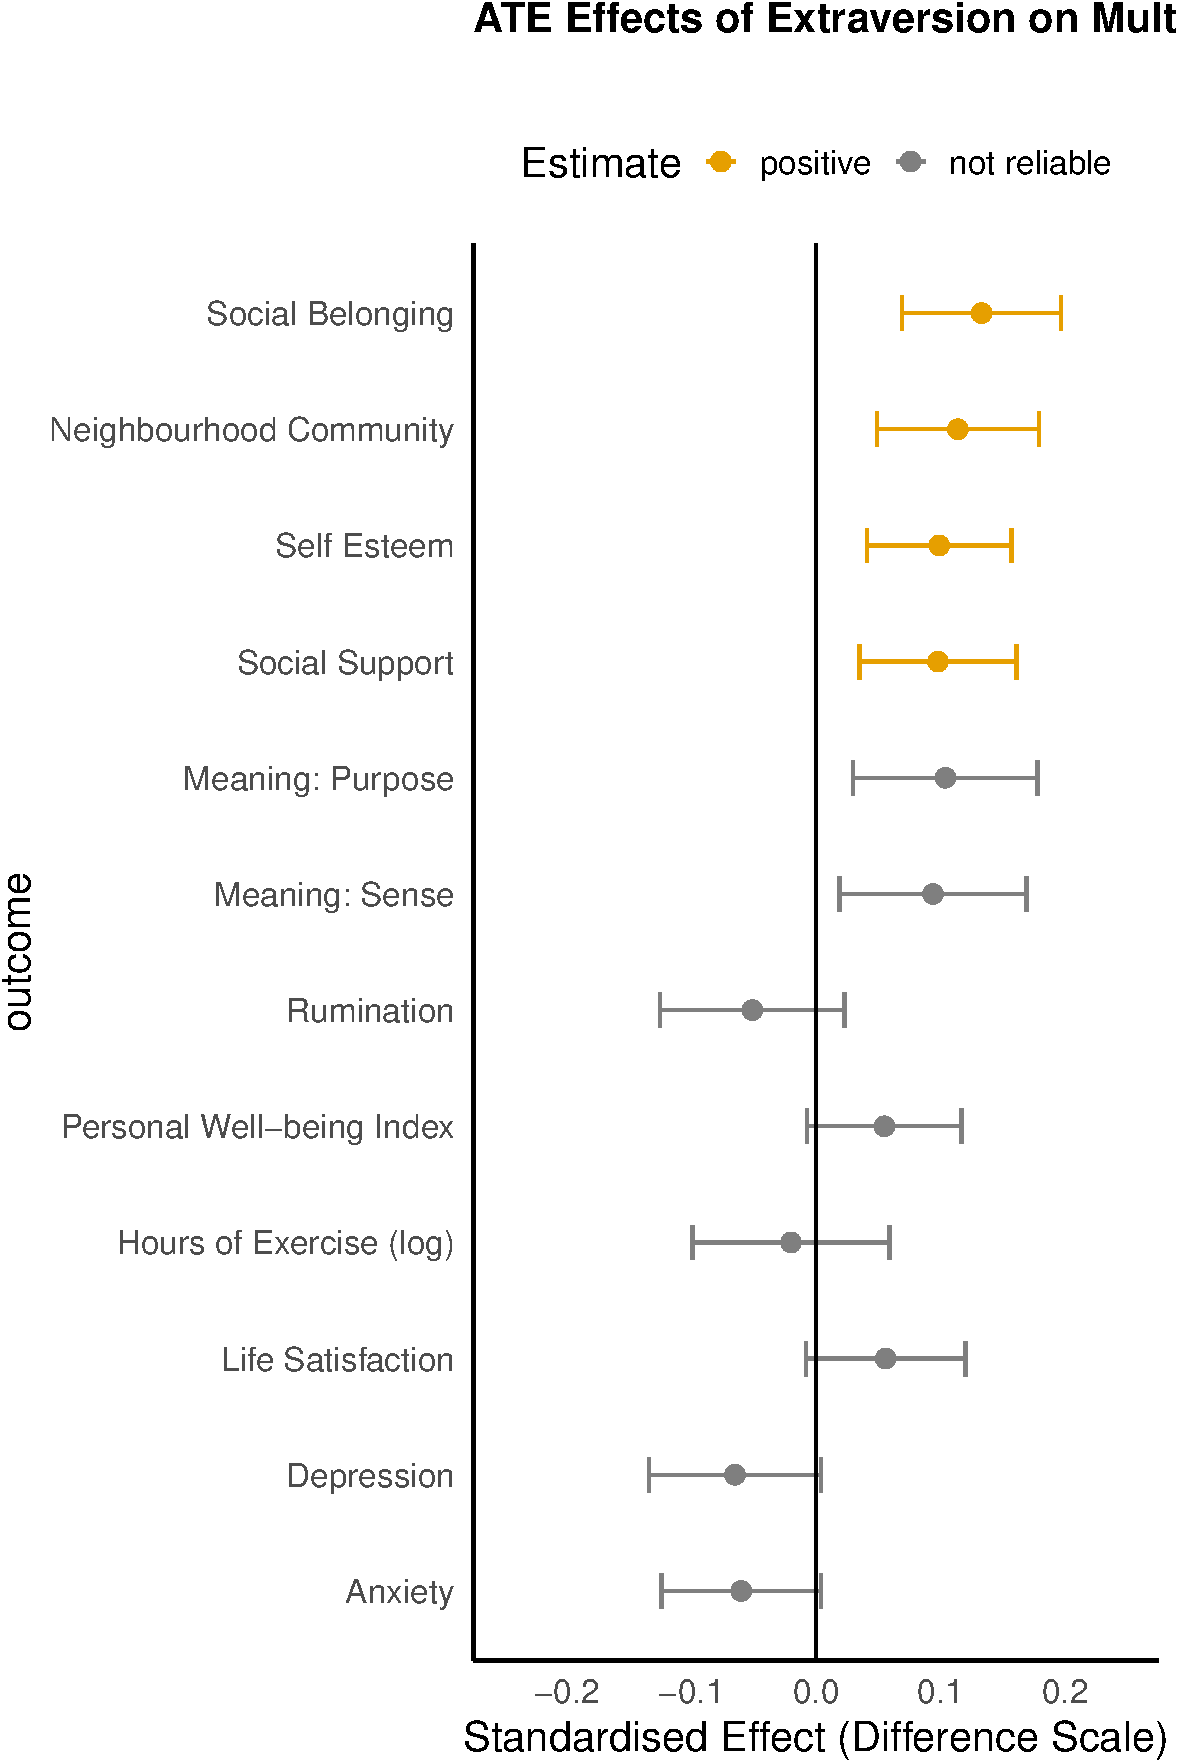
\includegraphics[keepaspectratio]{initial_quarto_document_files/figure-pdf/fig-ate-1.pdf}}

}

\caption{\label{fig-ate}Average Treatment Effects on Multi-dimensional
Wellbeing}

\end{figure}%

\newpage{}

\begin{longtable}[]{@{}
  >{\raggedright\arraybackslash}p{(\linewidth - 10\tabcolsep) * \real{0.3415}}
  >{\raggedright\arraybackslash}p{(\linewidth - 10\tabcolsep) * \real{0.1220}}
  >{\raggedright\arraybackslash}p{(\linewidth - 10\tabcolsep) * \real{0.1220}}
  >{\raggedright\arraybackslash}p{(\linewidth - 10\tabcolsep) * \real{0.1220}}
  >{\raggedright\arraybackslash}p{(\linewidth - 10\tabcolsep) * \real{0.1220}}
  >{\raggedright\arraybackslash}p{(\linewidth - 10\tabcolsep) * \real{0.1707}}@{}}

\caption{\label{tbl-outcomes}Average Treatment Effects on
Multi-dimensional Wellbeing}

\tabularnewline

\toprule\noalign{}
\begin{minipage}[b]{\linewidth}\raggedright
Outcome
\end{minipage} & \begin{minipage}[b]{\linewidth}\raggedright
ATE
\end{minipage} & \begin{minipage}[b]{\linewidth}\raggedright
2.5 \%
\end{minipage} & \begin{minipage}[b]{\linewidth}\raggedright
97.5 \%
\end{minipage} & \begin{minipage}[b]{\linewidth}\raggedright
E-Value
\end{minipage} & \begin{minipage}[b]{\linewidth}\raggedright
E-Value bound
\end{minipage} \\
\midrule\noalign{}
\endhead
\bottomrule\noalign{}
\endlastfoot
\textbf{Social Belonging} & \textbf{0.133} & \textbf{0.09} &
\textbf{0.177} & \textbf{1.51} & \textbf{1.39} \\
\textbf{Neighbourhood Community} & \textbf{0.114} & \textbf{0.07} &
\textbf{0.159} & \textbf{1.458} & \textbf{1.328} \\
\textbf{Self Esteem} & \textbf{0.099} & \textbf{0.06} & \textbf{0.139} &
\textbf{1.415} & \textbf{1.299} \\
\textbf{Social Support} & \textbf{0.098} & \textbf{0.055} &
\textbf{0.141} & \textbf{1.413} & \textbf{1.284} \\
\textbf{Meaning: Purpose} & \textbf{0.104} & \textbf{0.053} &
\textbf{0.154} & \textbf{1.43} & \textbf{1.278} \\
\textbf{Meaning: Sense} & \textbf{0.094} & \textbf{0.043} &
\textbf{0.145} & \textbf{1.401} & \textbf{1.244} \\
Depression & -0.065 & -0.112 & -0.017 & 1.315 & 1.146 \\
Anxiety & -0.06 & -0.104 & -0.016 & 1.3 & 1.141 \\
Life Satisfaction & 0.056 & 0.012 & 0.1 & 1.287 & 1.121 \\
Personal Well-being Index & 0.055 & 0.013 & 0.098 & 1.284 & 1.116 \\
Rumination & -0.051 & -0.102 & -0.001 & 1.271 & 1.012 \\
Hours of Exercise (log) & -0.02 & -0.074 & 0.034 & 1.155 & 1 \\

\end{longtable}

Confidence intervals were adjusted for multiple comparisons using
bonferroni correction (\(\alpha\) = 0.05). E‑values were also adjusted
using bonferroni correction (\(\alpha\) = 0.05).

The following outcomes showed reliable causal evidence (E‑value lower
bound \textgreater{} 1.2): - Social Belonging: 0.133(0.069,0.197); on
the original scale, 0.145 (0.075,0.215). E‑value bound = 1.329 -
Neighbourhood Community: 0.114(0.049,0.179); on the original scale,
0.179 (0.077,0.281). E‑value bound = 1.264 - Self Esteem:
0.099(0.041,0.157); on the original scale, 0.126 (0.052,0.2). E‑value
bound = 1.238 - Social Support: 0.098(0.035,0.161); on the original
scale, 0.11 (0.039,0.18). E‑value bound = 1.216

Confidence intervals were adjusted for multiple comparisons using
bonferroni correction (\(\alpha\) = 0.05). E‑values were also adjusted
using bonferroni correction (\(\alpha\) = 0.05). The following outcomes
showed reliable causal evidence (E‑value lower bound \textgreater{}
1.2): - \textbf{Social Belonging}: 0.125(0.064,0.186); on the original
scale, 0.136 (0.07,0.203). E‑value bound = 1.311 - \textbf{Neighbourhood
Community}: 0.119(0.052,0.186); on the original scale, 0.187
(0.082,0.292). E‑value bound = 1.273 - Social Support:
0.096(0.032,0.16); on the original scale, 0.107 (0.036,0.179). E‑value
bound = 1.203.

\newpage{}

\subsubsection{Heterogeneous Treatment
Effects}\label{heterogeneous-treatment-effects}

\paragraph{RATE AUTOC and RATE Qini}\label{rate-autoc-and-rate-qini}

\paragraph{Rate Test}\label{rate-test}

The RATE metric shows how much extra gain (or avoided loss) we achieve
by \textbf{targeting} instead of treating everyone identically.

\textbf{Technical note}: In code we always set
\texttt{policy\ =\ "treat\_best"}; for harmful exposures this is
interpreted as \emph{`treat-those-most-sensitive'} (i.e., prioritise
protection or withholding).

\begin{itemize}
\tightlist
\item
  \textbf{Beneficial exposure:} we rank by positive CATEs and deliver
  the exposure to those predicted to \textbf{benefit most}.
\item
  \textbf{Detrimental exposure:} we rank by increasingly
  \textbf{positive} CATEs (more predicted harm) and identify those who
  should be protected or withheld from the exposure.
\end{itemize}

Either way, a larger \textbf{absolute} RATE shows that a CATE-based
targeting rule `outperforms' a one-size-fits-all policy---by boosting
outcomes for beneficial exposures or -- in the case where we are explore
sensitivity to harm -- evaluating increasing harms for detrimental ones.

Recall we flipped Anxiety, Depression, Rumination so \textbf{`higher'
always tracks the analysis goal: higher = more benefit for beneficial
exposures, higher = more harm for detrimental exposures.}

Because we test several outcomes, RATE \emph{p}-values are adjusted with
Benjamini--Hochberg false-discovery-rate adjustment (q = 0.1) before we
decide whether heterogeneity is actionable.

\subsubsection{Comparison of targeting operating characteristic (TOC) by
rank average treatment effect (RATE): AUTOC vs
QINI}\label{comparison-of-targeting-operating-characteristic-toc-by-rank-average-treatment-effect-rate-autoc-vs-qini}

We applied two TOC by RATE methods to the same causal-forest \tau(x)
estimates:

\begin{itemize}
\item
  \textbf{AUTOC} intensifies focus on top responders via logarithmic
  weighting.
\item
  \textbf{QINI} balances effect size and prevalence via linear
  weighting.
\end{itemize}

We treated the RATE analysis as exploratory. All 12 outcomes were
prespecified. To flag promising signals we controlled the false
discovery rate at q=0.20.

When QINI and AUTOC disagree on positive RATE (only AUTOC yields a
positive RATE for \textbf{Hours of Exercise (log)}; only QINI yields a
positive RATE for Meaning: Sense), choose \textbf{QINI} to maximise
overall benefit or \textbf{AUTOC} to focus on top responders.

Refer to \hyperref[appendix-cate-validation]{Appendix E} for details.

\subparagraph{RATE AUTOC Results}\label{rate-autoc-results}

\subsubsection{Evidence for heterogeneous treatment effects (policy =
treat best responders) using
AUTOC}\label{evidence-for-heterogeneous-treatment-effects-policy-treat-best-responders-using-autoc}

AUTOC uses logarithmic weighting to focus treatment on top responders.
We treated the RATE analysis as exploratory. All 12 outcomes were
prespecified. To flag promising signals we controlled the false
discovery rate at q=0.20.

Positive RATE estimates for: \textbf{Hours of Exercise (log)}.

Estimates (\textbf{Hours of Exercise (log)}: 0.065 (95\% CI 0.018,
0.112)) show robust heterogeneity.

For outcomes with adjusted p-values not meeting the FDR threshold of q =
0.20 (Meaning: Sense, Rumination, Anxiety, Personal Well-being Index,
Self Esteem, Social Belonging, Social Support, Life Satisfaction,
Meaning: Purpose, Depression, Neighbourhood Community), evidence is
inconclusive.

\begin{figure}

\centering{

\pandocbounded{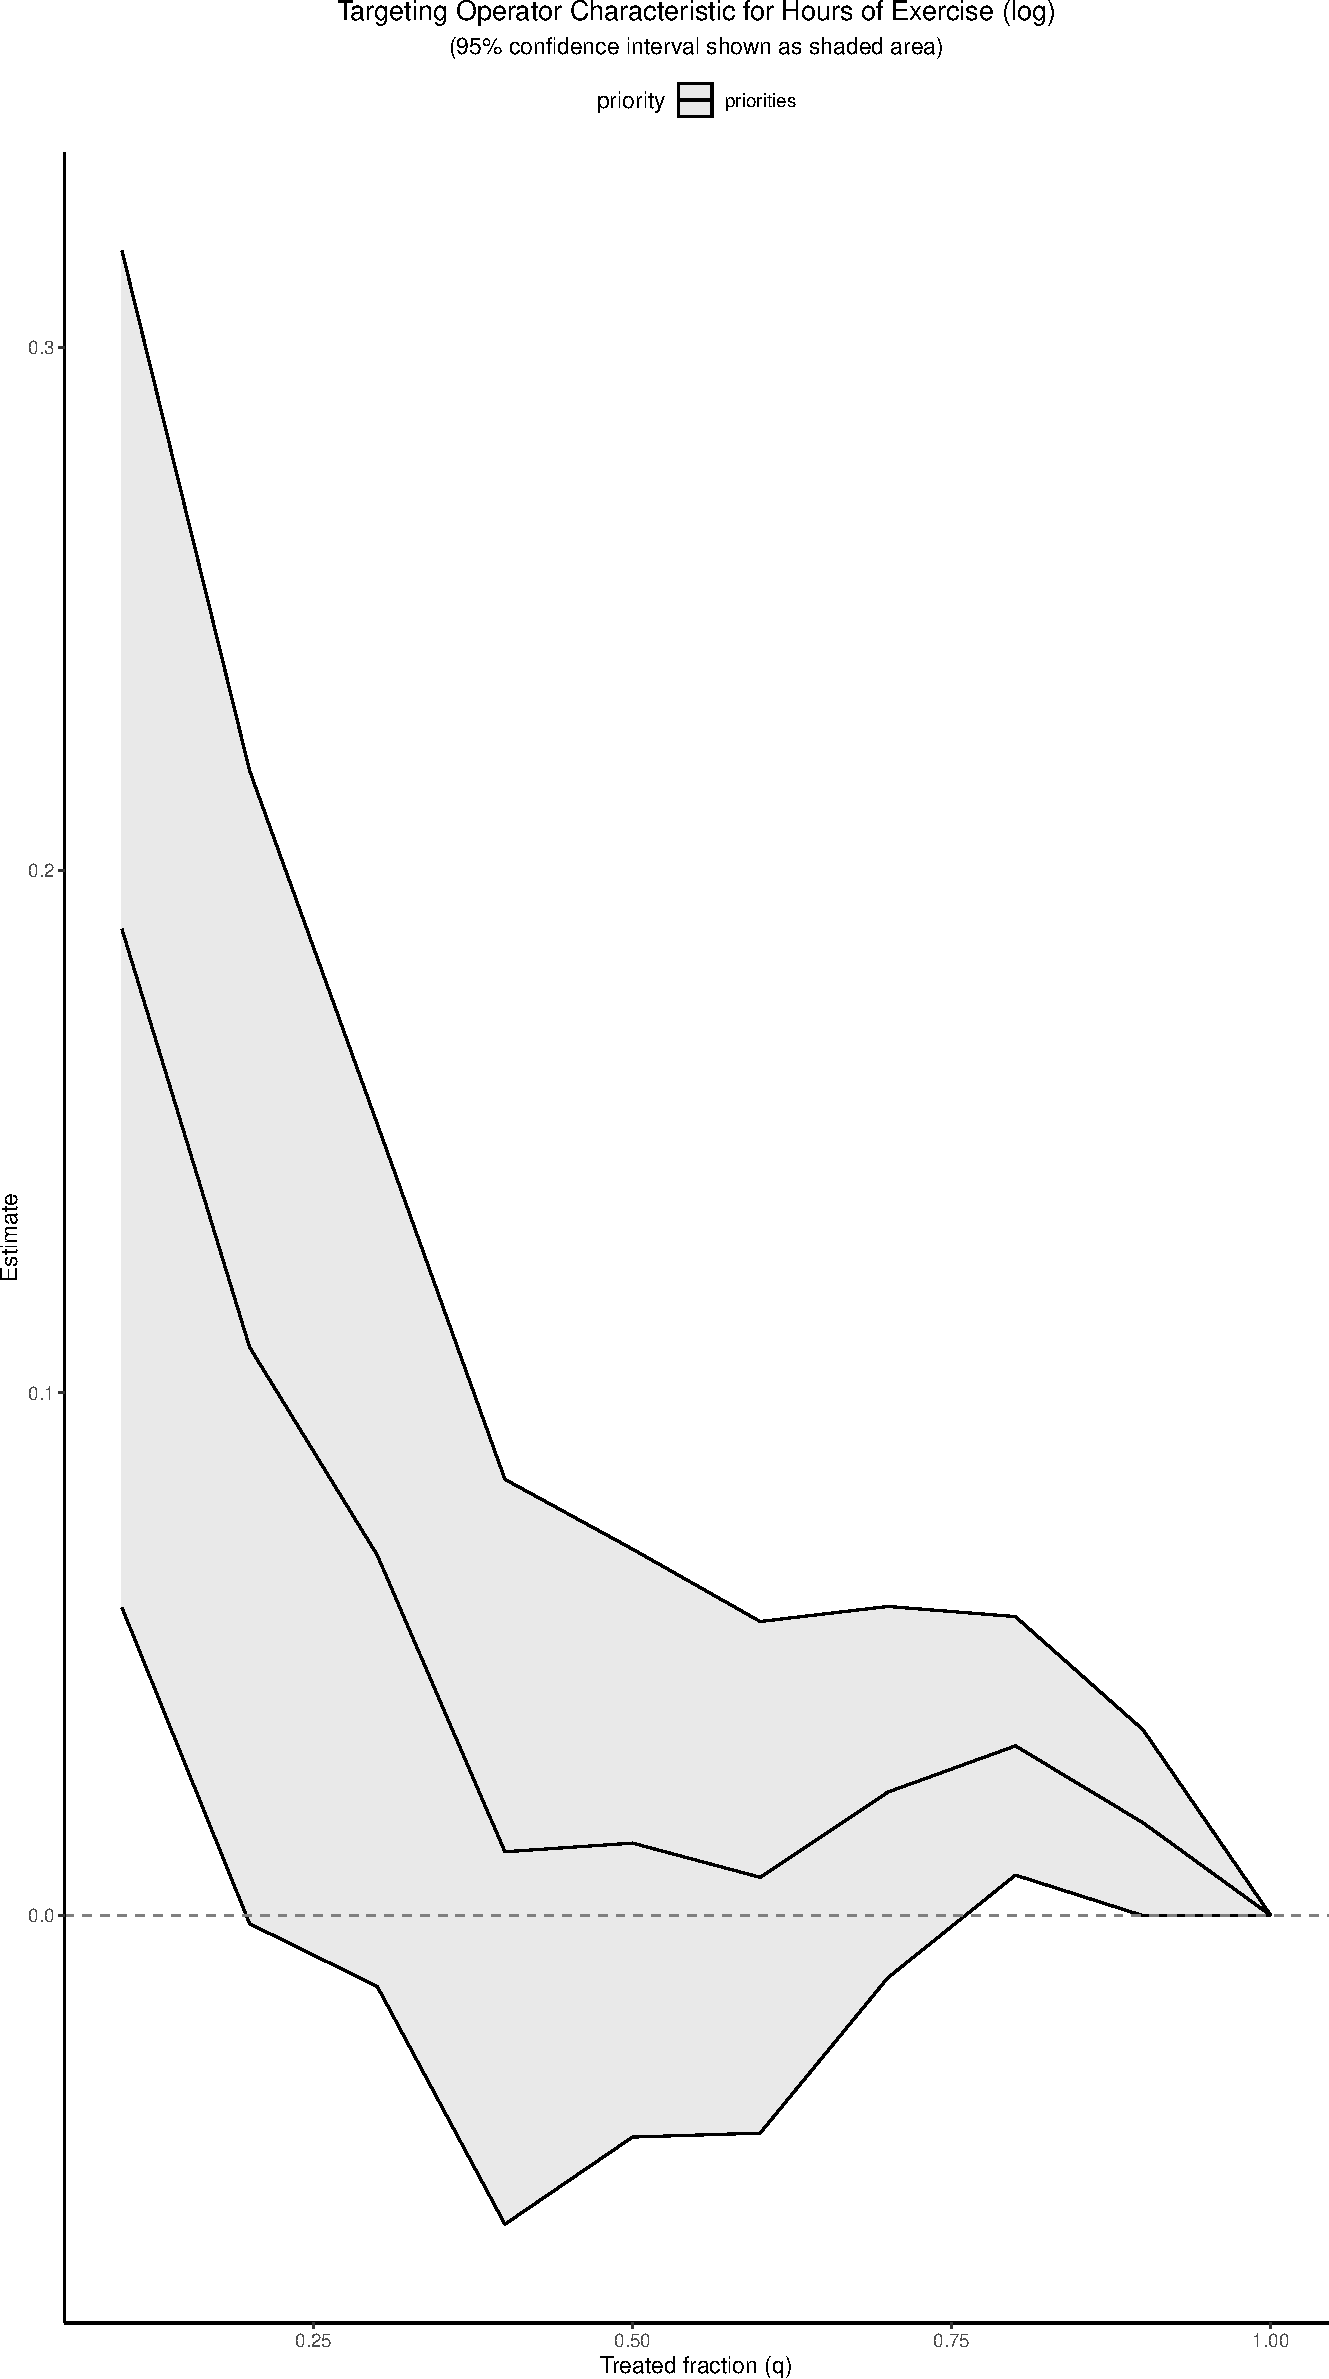
\includegraphics[keepaspectratio]{initial_quarto_document_files/figure-pdf/fig-rate-1-1.pdf}}

}

\caption{\label{fig-rate-1}RATE AUTOC Graphs}

\end{figure}%

Figure~\ref{fig-rate-1} presents the RATE AUTOC curve for Hours of
Exercise (log)

\subparagraph{RATE Qini Results}\label{rate-qini-results}

\subsubsection{Evidence for heterogeneous treatment effects (policy =
treat best responders) using
QINI}\label{evidence-for-heterogeneous-treatment-effects-policy-treat-best-responders-using-qini}

QINI uses linear weighting to balance effect size and prevalence. We
treated the RATE analysis as exploratory. All 12 outcomes were
prespecified. To flag promising signals we controlled the false
discovery rate at q=0.20.

Positive RATE estimates for: \textbf{Meaning: Sense}.

Estimates (\textbf{Meaning: Sense}: 0.020 (95\% CI 0.002, 0.038)) show
robust heterogeneity.

Negative RATE estimates for: Neighbourhood Community.

Estimates (Neighbourhood Community: -0.026 (95\% CI -0.042, -0.010))
caution against CATE prioritisation.

For outcomes with adjusted p-values not meeting the FDR threshold of q =
0.20 (Hours of Exercise (log), Personal Well-being Index, Anxiety, Self
Esteem, Social Support, Life Satisfaction, Social Belonging, Rumination,
Meaning: Purpose, Depression), evidence is inconclusive.

\paragraph{QINI Curve Analysis}\label{qini-curve-analysis}

\paragraph{Qini Curves}\label{qini-curves}

The Qini curve shows the cumulative \textbf{gain} as we expand a
targeting rule down the CATE ranking.

\begin{itemize}
\tightlist
\item
  \textbf{Beneficial exposure:} we add individuals from the top positive
  CATEs downward; the baseline is `expose everyone.'
\item
  \textbf{Detrimental exposure:} we first flip outcome direction (so
  higher values represent \textbf{more harm}; see Anxiety, Depression,
  Rumination), then \emph{add} the exposure starting with individuals
  whose CATEs show the \textbf{greated harm}, gradually including those
  predicted to be more resistant to harm; the baseline is `expose
  everyone.' The curve therefore quantifies the harm by when those most
  suceptible to harm are exposed.
\end{itemize}

If the Qini curve stays above its baseline, a targeted policy increases
the outcome more than a one-size-fits-all alternative. (Outcome
directions were flipped where needed---Anxiety, Depression,
Rumination---so the positively valenced exposures always have positively
valanced outcomes and negative exposures always have negatively valenced
outcomes.)

We computed the cumulative benefits as we increase the treated fraction
by prioritising conditional average treatment effects (CATE) at two
different spend levels: 20\% of a total budget and 50\% of a total
budget, where the contrast is no priority assignment. \textbf{Meaning
Sense} At 20\% spend: CATE prioritisation is beneficial (diff: 0.08
{[}95\% CI: 0.04, 0.12{]}). At 50\% spend: CATE prioritisation is
beneficial (diff: 0.07 {[}95\% CI: 0.02, 0.12{]}).

Table~\ref{tbl-qini} presents results for our Qini curve analysis at
different spend rates.

\begin{longtable}[]{@{}lll@{}}

\caption{\label{tbl-qini}Qini Curve Results}

\tabularnewline

\toprule\noalign{}
Model & Spend 20\% & Spend 50\% \\
\midrule\noalign{}
\endhead
\bottomrule\noalign{}
\endlastfoot
Meaning Sense & \textbf{0.08 {[}0.04, 0.12{]}} & \textbf{0.07 {[}0.02,
0.12{]}} \\

\end{longtable}

Figure~\ref{fig-qini-1} presents the Qini curve for Meaning: Sense

\begin{figure}

\centering{

\pandocbounded{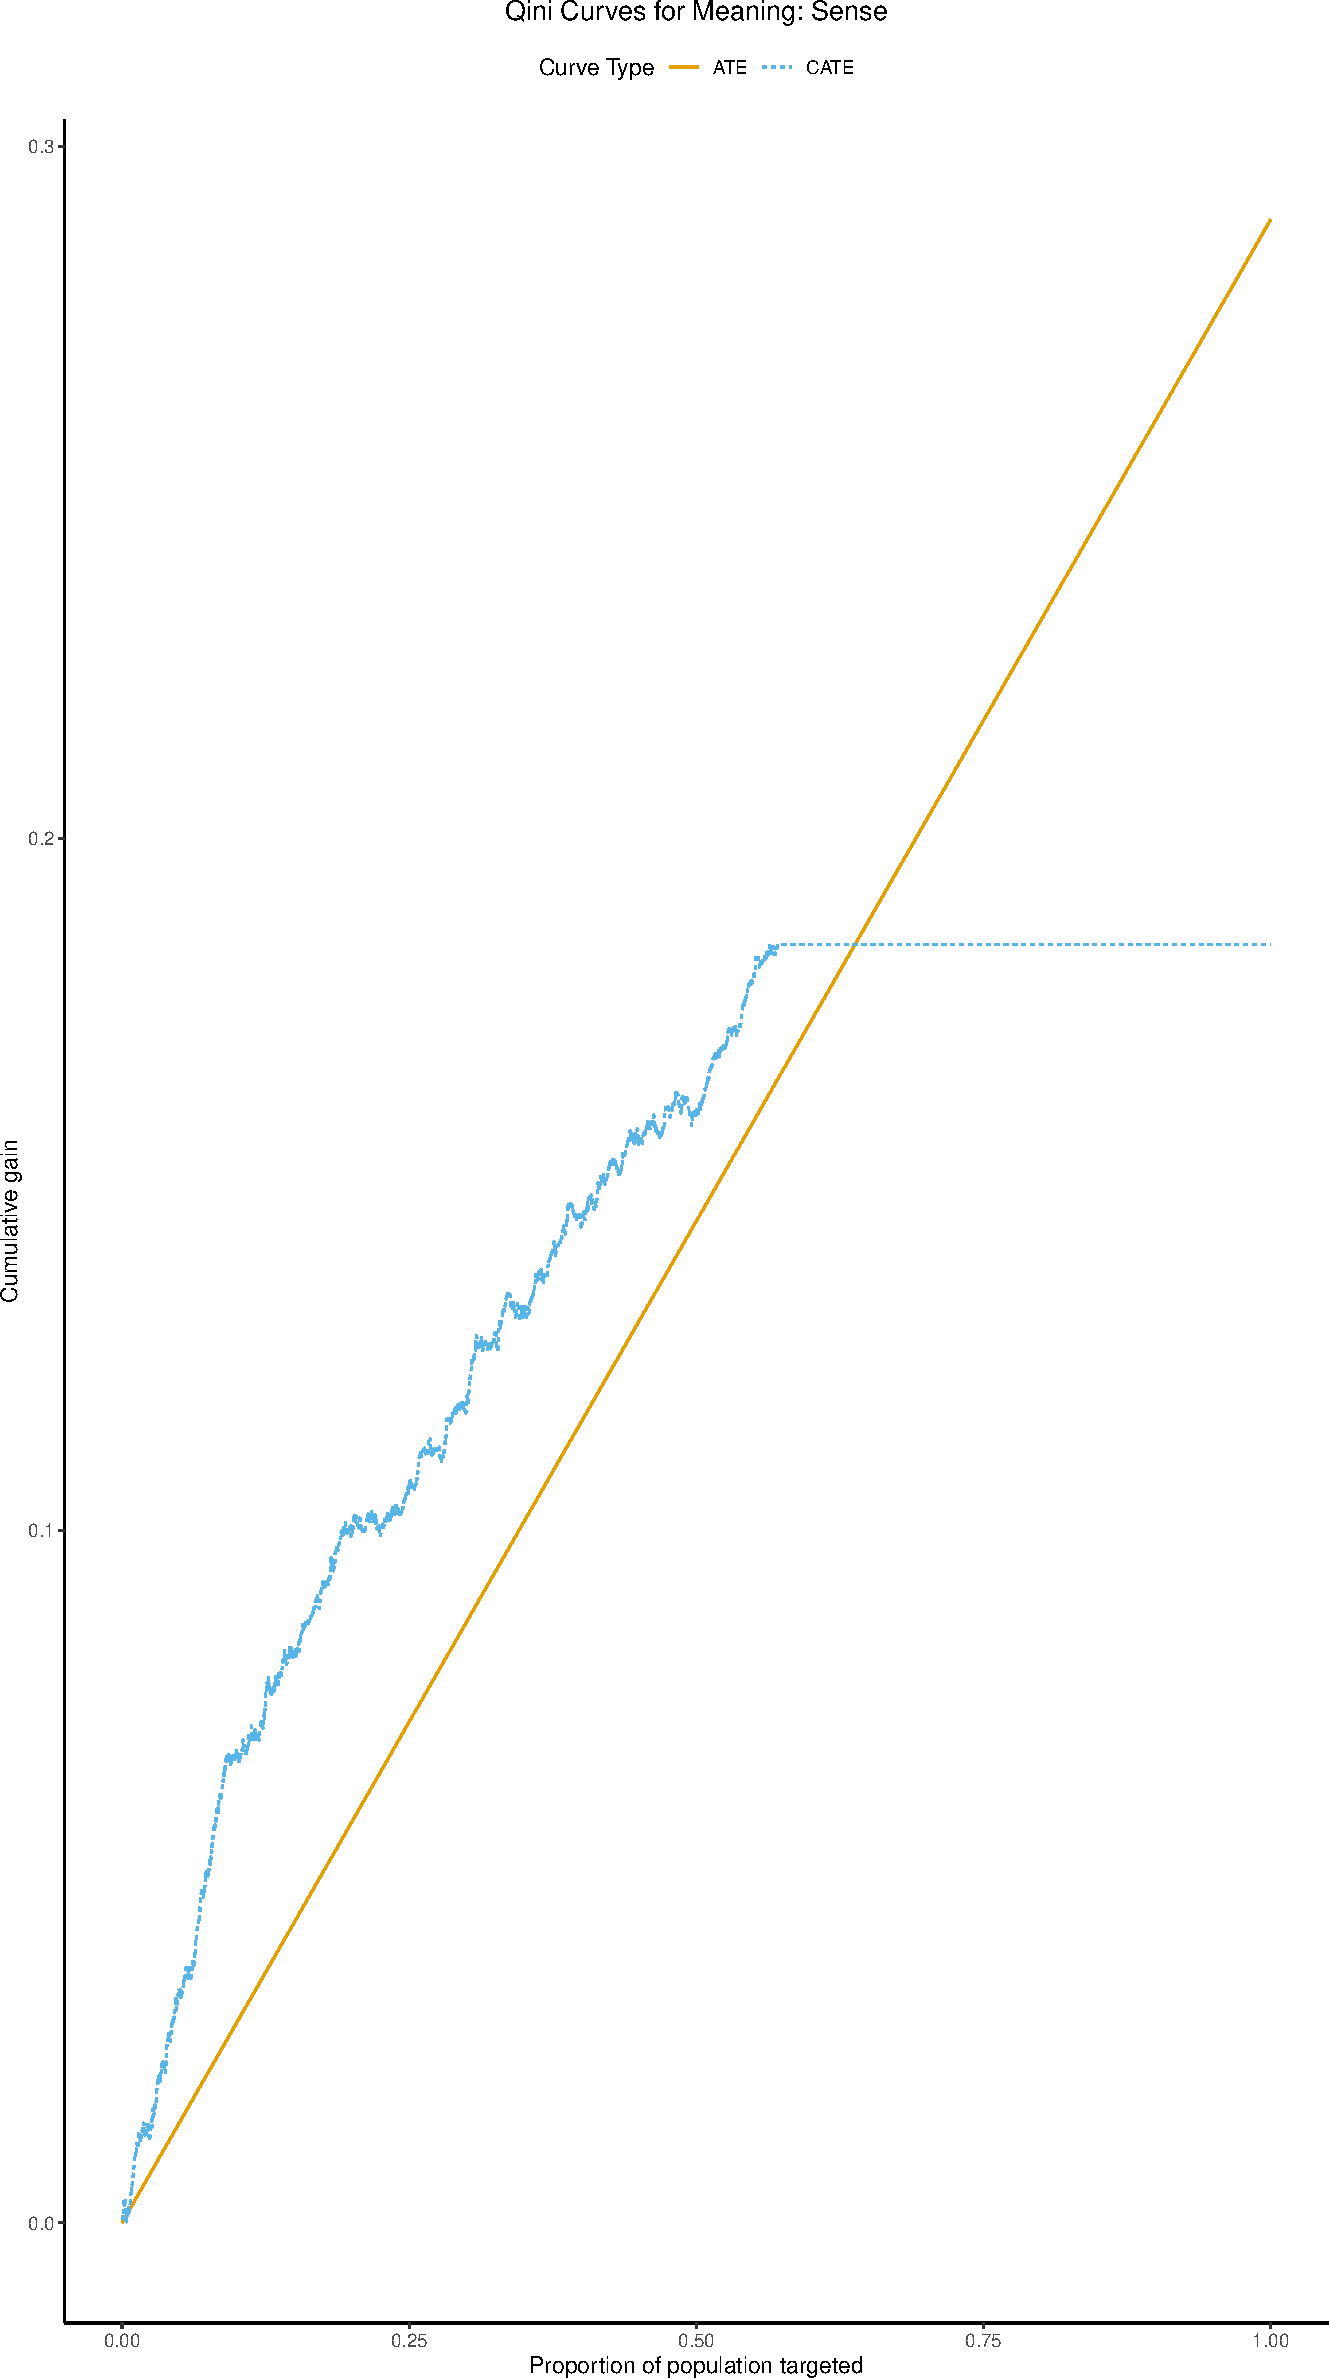
\includegraphics[keepaspectratio]{initial_quarto_document_files/figure-pdf/fig-qini-1-1.pdf}}

}

\caption{\label{fig-qini-1}Qini Graph}

\end{figure}%

\newpage{}

\paragraph{Decision Rules (Who is Most Sensitive to
Treatment?)}\label{decision-rules-who-is-most-sensitive-to-treatment}

\paragraph{Policy Trees}\label{policy-trees}

We used policy trees (\citeproc{ref-athey2021}{Athey \& Wager, 2021a},
\citeproc{ref-athey_2021_policy_tree_econometrica}{2021b};
\citeproc{ref-policytree_package_2024}{Sverdrup et al., 2024}) to find
straightforward `if-then' rules for who benefits most from treatment,
based on participant characteristics. Because we flipped some measures,
a higher predicted effect always means greater improvement. Policy trees
can uncover small but important subgroups whose treatment responses
stand out, even when the overall differences might be modest.

\begin{figure}

\centering{

\pandocbounded{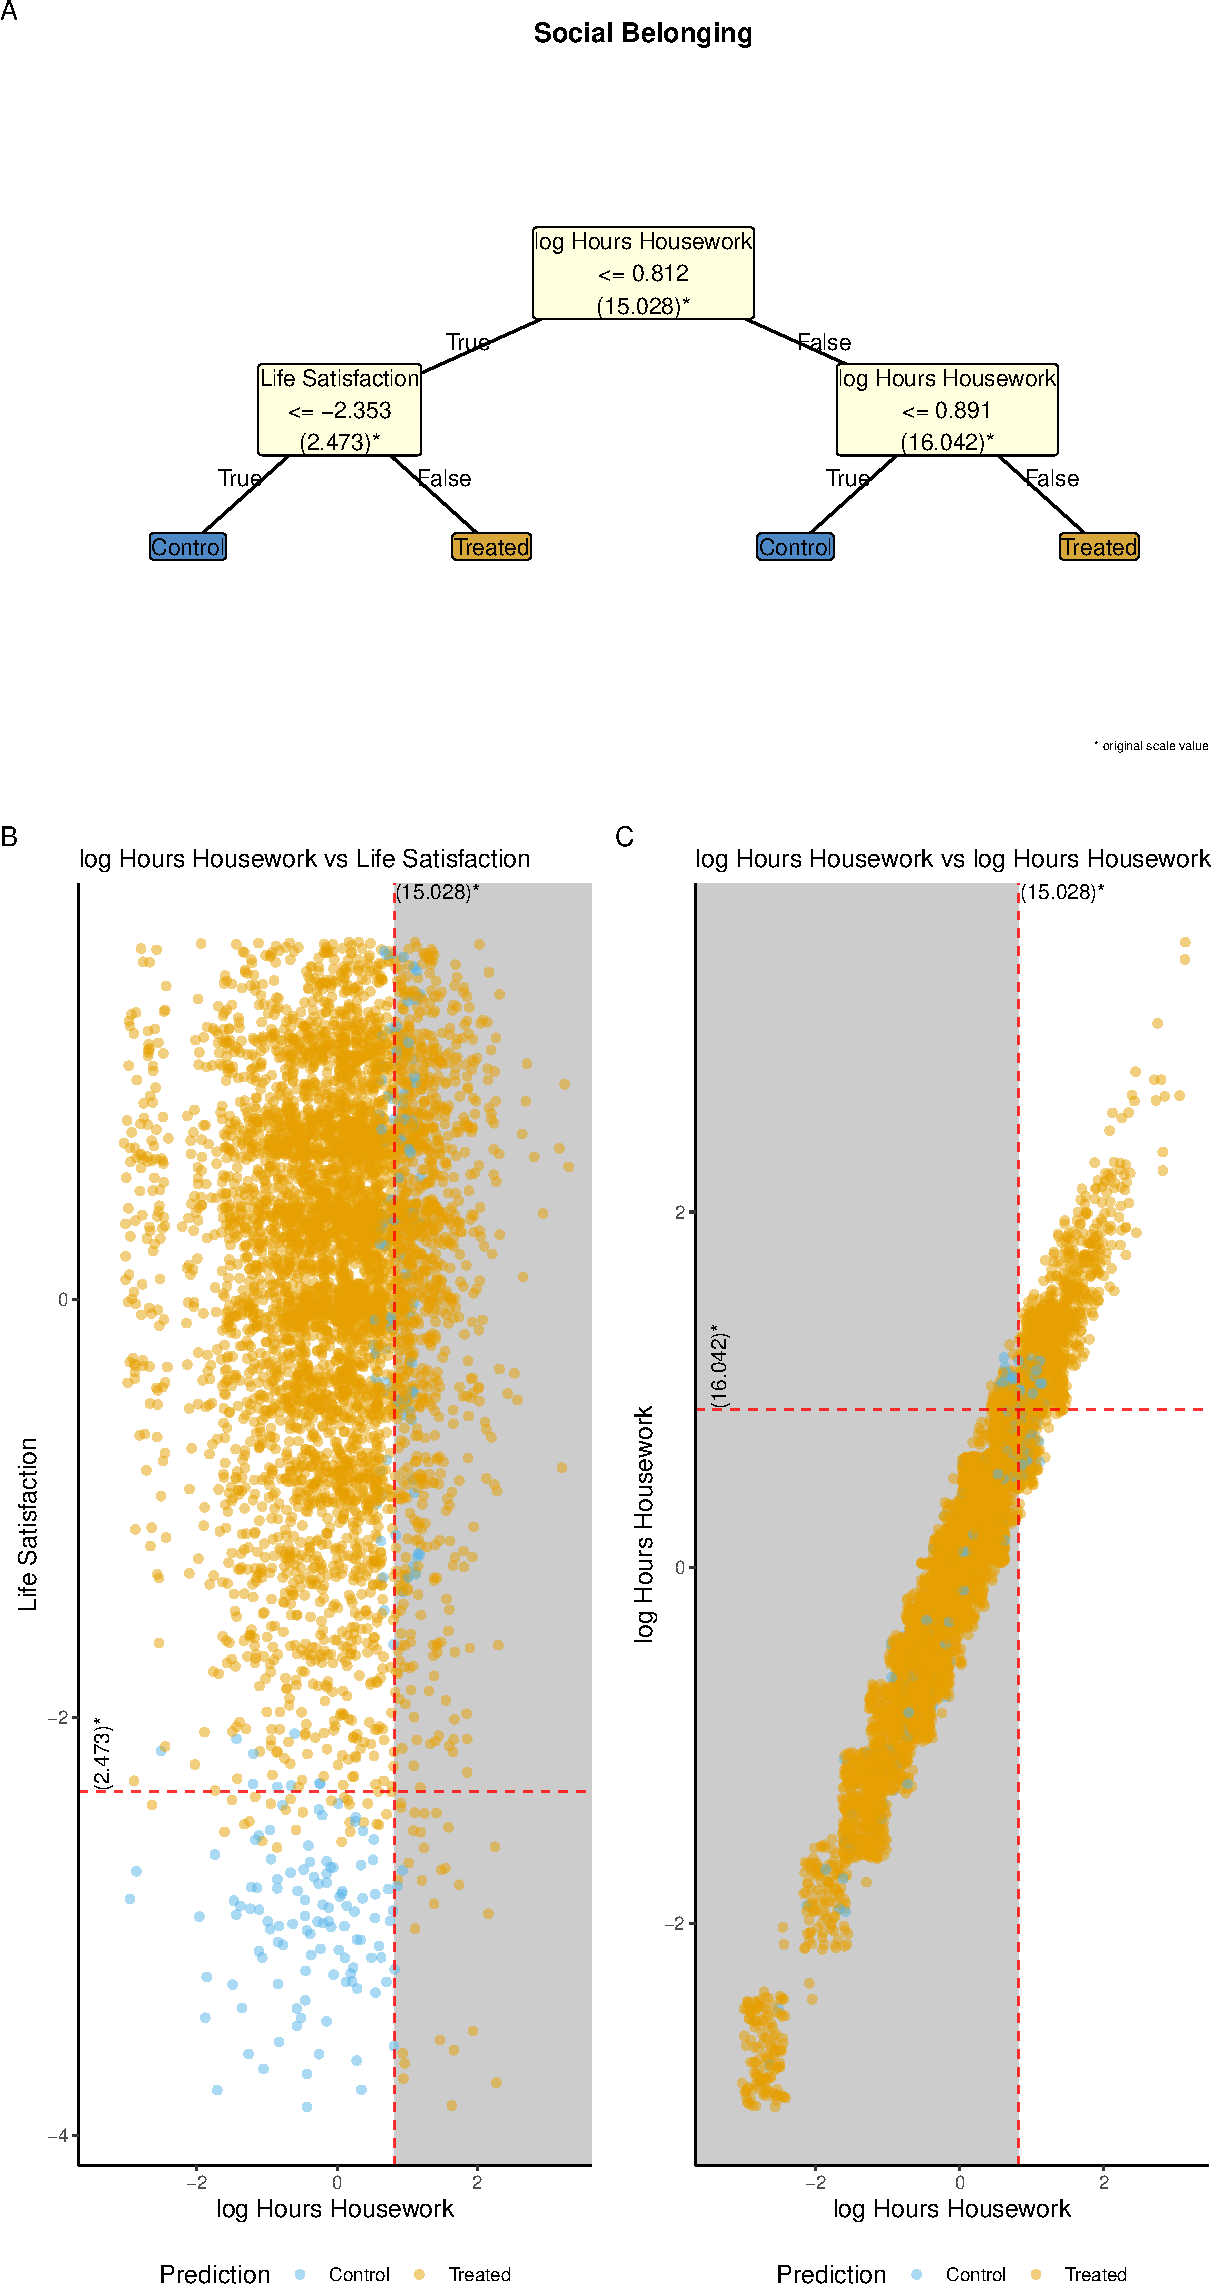
\includegraphics[keepaspectratio]{initial_quarto_document_files/figure-pdf/fig-policy-1-1.pdf}}

}

\caption{\label{fig-policy-1}Decision Tree: \{glued\_name\_policy\_1\}}

\end{figure}%

\begin{figure}

\centering{

\pandocbounded{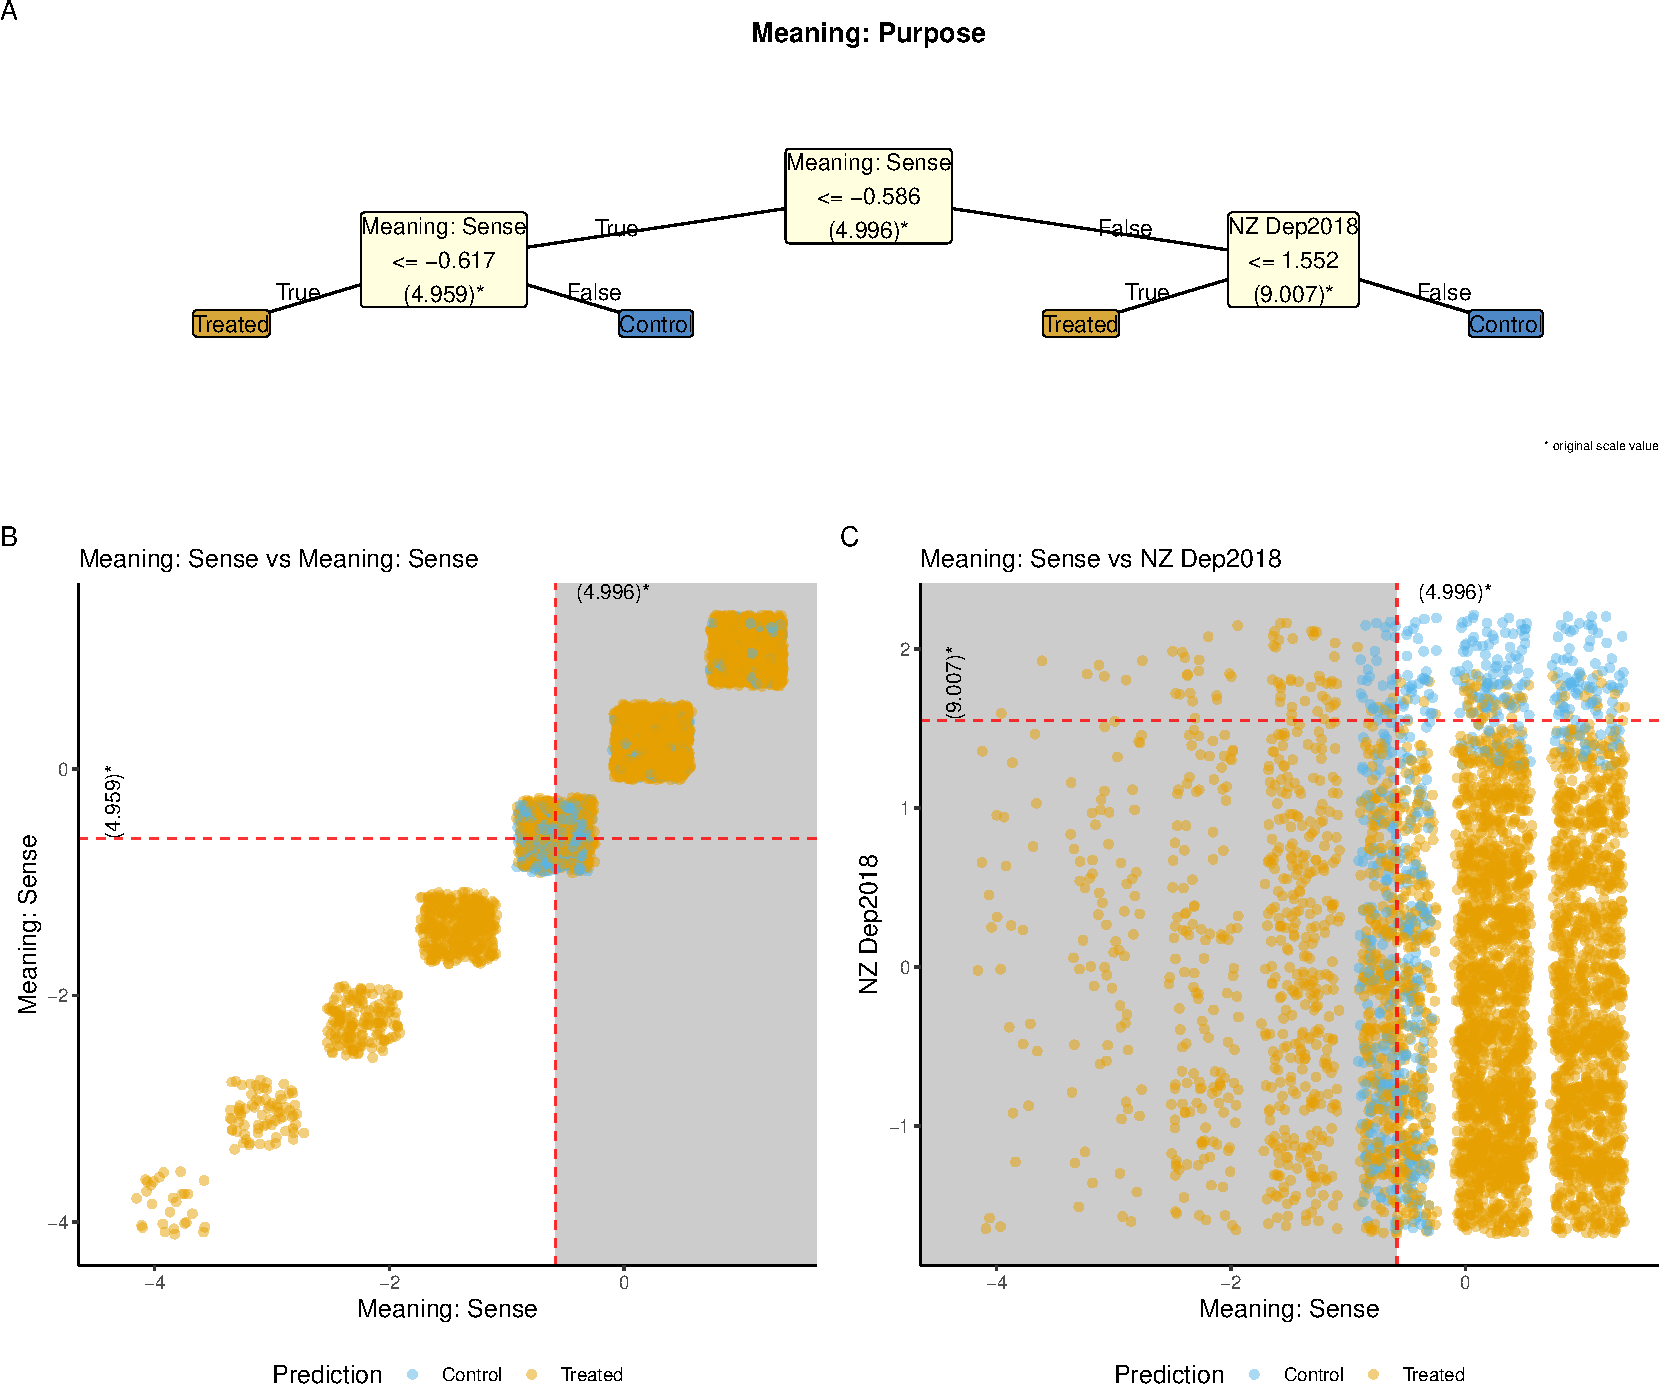
\includegraphics[keepaspectratio]{initial_quarto_document_files/figure-pdf/fig-policy-2-1.pdf}}

}

\caption{\label{fig-policy-2}Decision Tree: \{glued\_name\_policy\_2\}}

\end{figure}%

\subsubsection{Policy Tree Interpretations (depth
2)}\label{policy-tree-interpretations-depth-2}

A shallow policy tree recommends actions based on two splits for
depth=2, or one split for depth=1. We trained on 50\% of the data and
evaluated on the rest.

\textbf{Findings for log Hours Exercise:}

Split 1: Meaning Sense ≤ 0.201 (original: 5.953). Within that subgroup,
split 2a: log Hours Commute ≤ 0.346 (original: 4.983), →
\textbf{Control}; log Hours Commute \textgreater{} 0.346 (original:
4.983) → \textbf{Treated}.

Split 2: Meaning Sense \textgreater{} 0.201 (original: 5.953). Within
that subgroup, split 2b: log Hours Commute ≤ 0.543 (original: 6.044), →
\textbf{Treated}; log Hours Commute \textgreater{} 0.543 (original:
6.044) → \textbf{Control}.

\textbf{Findings for Meaning Sense:}

Split 1: log Household Inc ≤ 0.15 (original: 100000.015). Within that
subgroup, split 2a: Age ≤ 0.612 (original: 57), → \textbf{Treated}; Age
\textgreater{} 0.612 (original: 57) → \textbf{Control}.

Split 2: log Household Inc \textgreater{} 0.15 (original: 100000.015).
Within that subgroup, split 2b: log Hours Exercise ≤ -0.543 (original:
1.965), → \textbf{Control}; log Hours Exercise \textgreater{} -0.543
(original: 1.965) → \textbf{Treated}.

\newpage{} \#\# Planned Subgroup Comparisons (Optional)

Based on theoretical findings we expected that the effects of
\{name\_exposure\} would vary by
age\ldots{}Figure~\ref{fig-planned-comparison} and
Table~\ref{tbl-planned-comparison}

\begin{figure}

\centering{

\pandocbounded{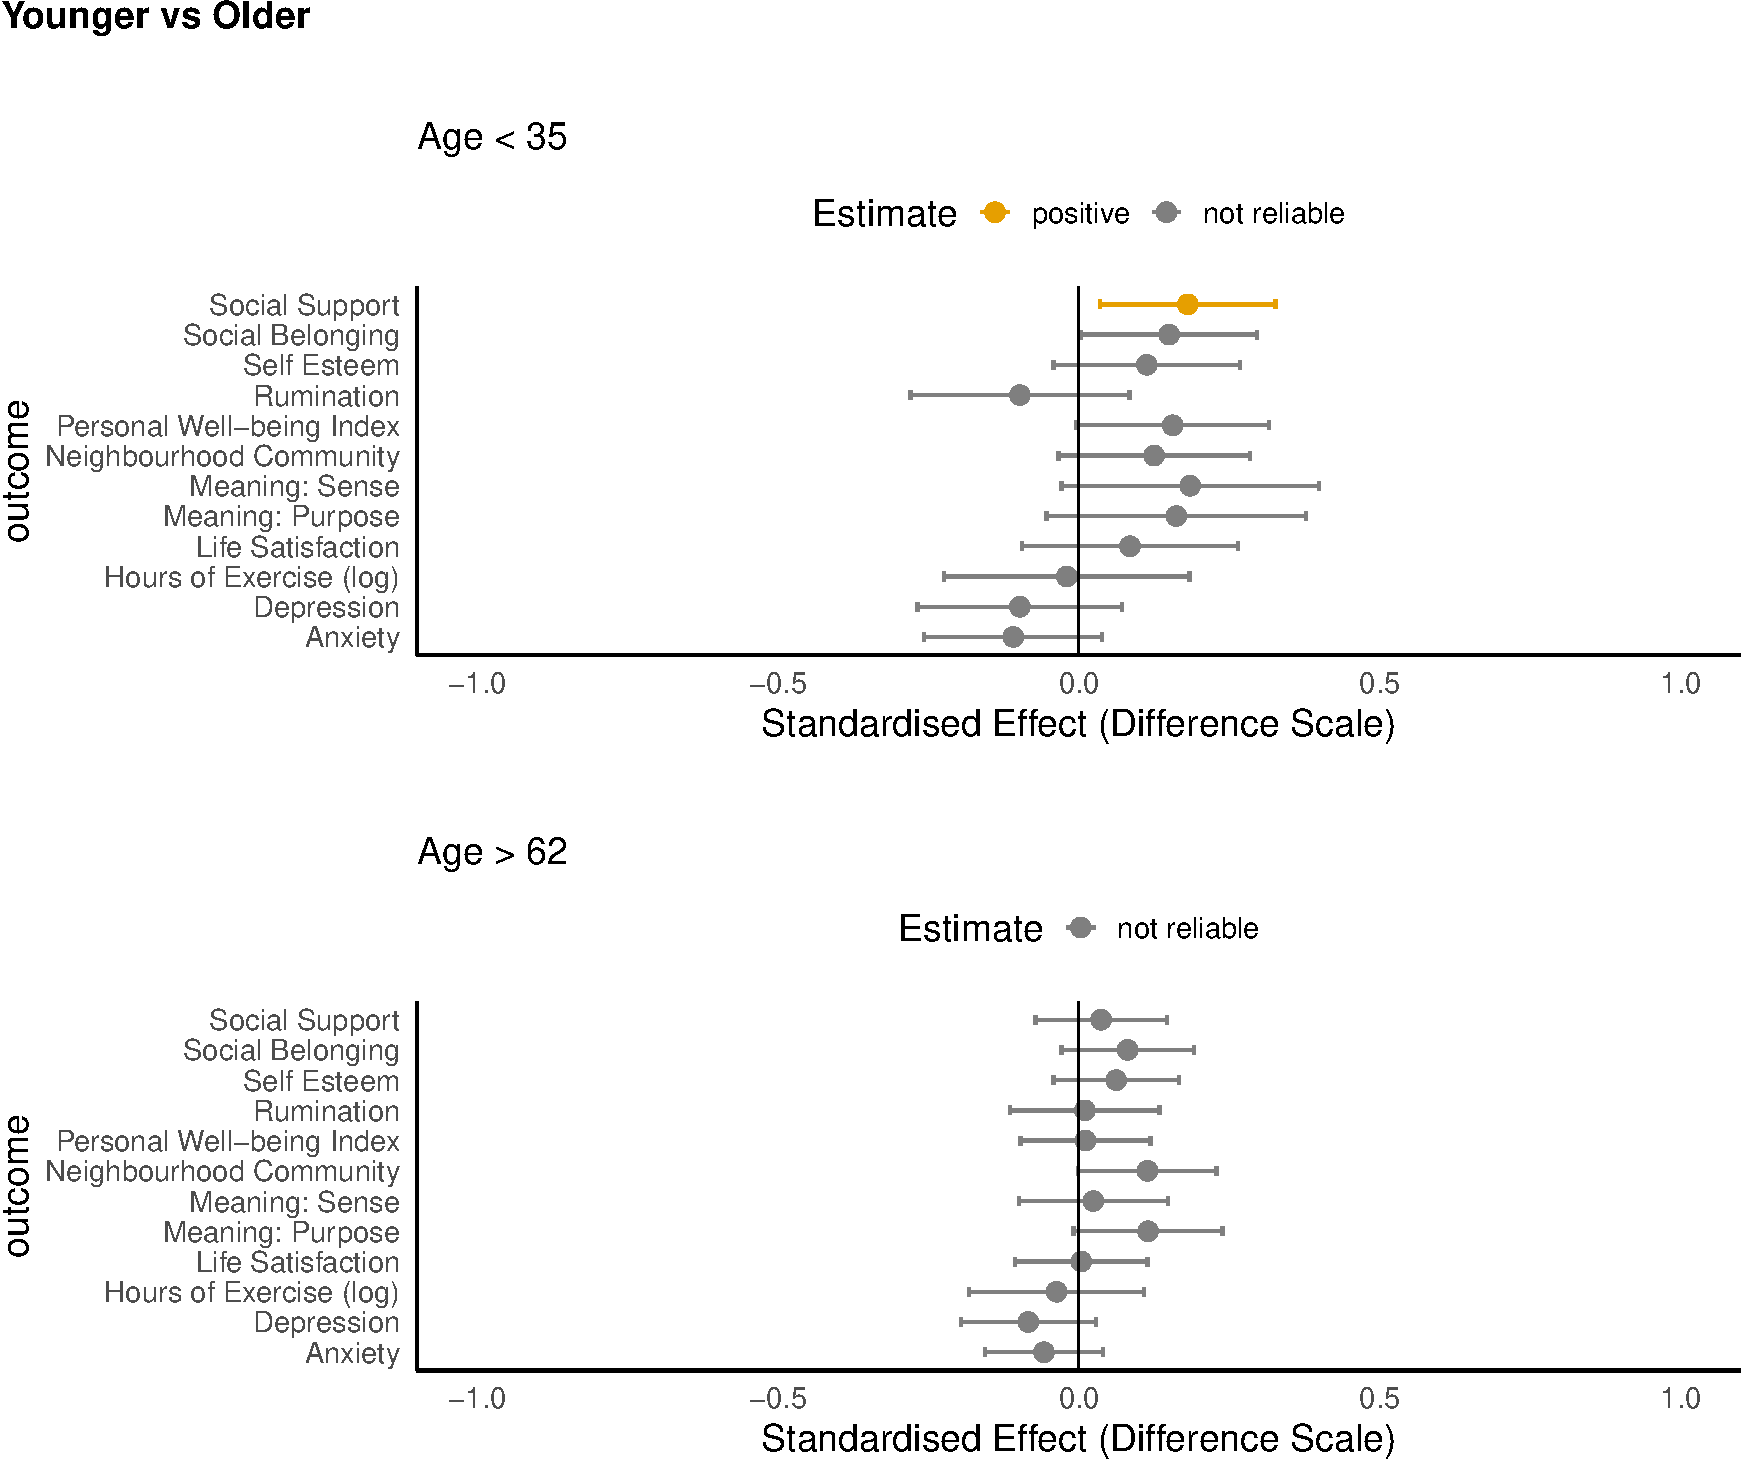
\includegraphics[keepaspectratio]{initial_quarto_document_files/figure-pdf/fig-planned-comparison-1.pdf}}

}

\caption{\label{fig-planned-comparison}Planned Comparison Plot}

\end{figure}%

\begin{longtable}[]{@{}ll@{}}

\caption{\label{tbl-planned-comparison}Planned Comparison Table}

\tabularnewline

\toprule\noalign{}
Outcomes & Group Differences \\
\midrule\noalign{}
\endhead
\bottomrule\noalign{}
\endlastfoot
Social Support & \textbf{-0.144 {[}-0.269, -0.019{]}} \\
Social Belonging & -0.069 {[}-0.194, 0.056{]} \\
Self Esteem & -0.051 {[}-0.179, 0.077{]} \\
Rumination & 0.108 {[}-0.043, 0.259{]} \\
Personal Well-being Index & \textbf{-0.145 {[}-0.277, -0.013{]}} \\
Neighbourhood Community & -0.011 {[}-0.146, 0.124{]} \\
Meaning: Sense & -0.161 {[}-0.330, 0.008{]} \\
Meaning: Purpose & -0.047 {[}-0.218, 0.124{]} \\
Life Satisfaction & -0.081 {[}-0.225, 0.063{]} \\
Hours of Exercise (log) & -0.017 {[}-0.188, 0.154{]} \\
Depression & 0.014 {[}-0.125, 0.153{]} \\
Anxiety & 0.051 {[}-0.070, 0.172{]} \\

\end{longtable}

We found reliable treatment-effect differences comparing People Over 62
Years Old to People Under 35 Years Old for Social Support (People Over
62 Years Old vs People Under 35 Years Old): \(\delta\) = -0.144
{[}-0.269, -0.019{]} and Personal Well-being Index (People Over 62 Years
Old vs People Under 35 Years Old): \(\delta\) = -0.145 {[}-0.277,
-0.013{]}. We did not find reliable differences for all other outcomes.

\newpage{}

\subsection{Discussion}\label{discussion}

\newpage{}

\subsection{Appendix A: Measures}\label{appendix-measures}

\subsubsection{Measures}\label{measures}

\paragraph{Baseline Covariate
Measures}\label{baseline-covariate-measures}

\subsubsection{Baseline Covariates}\label{baseline-covariates}

\paragraph{Age}\label{age}

\emph{What is your date of birth?}

We asked participants' ages in an open-ended question (``What is your
age?'' or ``What is your date of birth'').
(\citeproc{ref-string_is}{\textbf{string\_is?}} Developed for the
NZAVS.)

\paragraph{Agreeableness}\label{agreeableness}

\emph{I sympathize with others' feelings.} \emph{I am not interested in
other people's problems.} \emph{I feel others' emotions.} \emph{I am not
really interested in others (reversed).}

Mini-IPIP6 Agreeableness dimension: (i) I sympathize with others'
feelings. (ii) I am not interested in other people's problems. (r) (iii)
I feel others' emotions. (iv) I am not really interested in others. (r)
(\citeproc{ref-sibley2011}{Sibley et al., 2011})

\paragraph{Alcohol Frequency}\label{alcohol-frequency}

\emph{``How often do you have a drink containing alcohol?''}

Participants could chose between the following responses: `(1 = Never -
I don't drink, 2 = Monthly or less, 3 = Up to 4 times a month, 4 = Up to
3 times a week, 5 = 4 or more times a week, 6 = Don't know)'
(\citeproc{ref-Ministry_of_Health_2013}{Health, 2013})

\paragraph{Alcohol Intensity}\label{alcohol-intensity}

\emph{``How many drinks containing alcohol do you have on a typical day
when drinking alcohol? (number of drinks on a typical day when
drinking)''}

Participants responded using an open-ended box.
(\citeproc{ref-Ministry_of_Health_2013}{Health, 2013})

\paragraph{Social Belonging}\label{social-belonging}

\emph{Know that people in my life accept and value me.} \emph{Feel like
an outsider (reversed).} \emph{Know that people around me share my
attitudes and beliefs.}

We assessed felt belongingness with three items adapted from the Sense
of Belonging Instrument (Hagerty \& Patusky, 1995): (1) ``Know that
people in my life accept and value me''; (2) ``Feel like an outsider'';
(3) ``Know that people around me share my attitudes and beliefs''.
Participants responded on a scale from 1 (Very Inaccurate) to 7 (Very
Accurate). The second item was reversely coded.
(\citeproc{ref-hagerty1995}{Hagerty \& Patusky, 1995})

\paragraph{Born in Nz}\label{born-in-nz}

\emph{Where were you born? (please be specific, e.g., which town/city?)}

Coded binary (1 = New Zealand; 0 = elsewhere.)
(\citeproc{ref-string_is}{\textbf{string\_is?}} Developed for the
NZAVS.)

\paragraph{Conscientiousness}\label{conscientiousness}

\emph{I get chores done right away.} \emph{I like order.} \emph{I make a
mess of things.} \emph{I often forget to put things back in their proper
place.}

Mini-IPIP6 Conscientiousness dimension: (i) I get chores done right
away. (ii) I like order. (iii) I make a mess of things. (r) (iv) I often
forget to put things back in their proper place. (r)
(\citeproc{ref-sibley2011}{Sibley et al., 2011})

\paragraph{Education Level}\label{education-level}

\emph{What is your highest level of qualification?}

We asked participants, ``What is your highest level of qualification?''.
We coded participans highest finished degree according to the New
Zealand Qualifications Authority. Ordinal-Rank 0-10 NZREG codes (with
overseas school qualifications coded as Level 3, and all other ancillary
categories coded as missing)
(\citeproc{ref-string_is}{\textbf{string\_is?}} Developed for the
NZAVS.)

\paragraph{Employed}\label{employed}

\emph{Are you currently employed (This includes self-employed of casual
work)?}

Binary response: (0 = No, 1 = Yes)
(\citeproc{ref-string_is}{\textbf{string\_is?}} Stats NZ Census
Question)

\paragraph{Ethnicity}\label{ethnicity}

\emph{Which ethnic group(s) do you belong to?}

Coded string: (1 = New Zealand European; 2 = Māori; 3 = Pacific; 4 =
Asian) (\citeproc{ref-string_is}{\textbf{string\_is?}} NZ Census
coding.)

\paragraph{Disability Status}\label{disability-status}

\emph{Do you have a health condition or disability that limits you and
that has lasted for 6+ months?}

We assessed disability with a one-item indicator adapted from Verbrugge
(1997). It asks, ``Do you have a health condition or disability that
limits you and that has lasted for 6+ months?'' (1 = Yes, 0 = No).
(\citeproc{ref-verbrugge1997}{Verbrugge, 1997})

\paragraph{Log Hours with Children}\label{log-hours-with-children}

\emph{Hours spent\ldots looking after children.}

We took the natural log of the response + 1.
(\citeproc{ref-sibley2011}{Sibley et al., 2011})

\paragraph{Log Hours Commuting}\label{log-hours-commuting}

\emph{Hours spent\ldots travelling/commuting.}

We took the natural log of the response + 1.
(\citeproc{ref-string_is}{\textbf{string\_is?}} Developed for the
NZAVS.)

\paragraph{Log Hours of Exercise}\label{log-hours-of-exercise}

\emph{Hours spent\ldots exercising/physical activity.}

We took the natural log of the response + 1.
(\citeproc{ref-sibley2011}{Sibley et al., 2011})

\paragraph{Log Hours on Housework}\label{log-hours-on-housework}

\emph{Hours spent\ldots housework/cooking.}

We took the natural log of the response + 1.
(\citeproc{ref-sibley2011}{Sibley et al., 2011})

\paragraph{Log Household Income}\label{log-household-income}

\emph{Please estimate your total household income (before tax) for the
year XXXX.}

We took the natural log of the response + 1.
(\citeproc{ref-string_is}{\textbf{string\_is?}} Developed for the
NZAVS.)

\paragraph{Male}\label{male}

\emph{We asked participants' gender in an open-ended question: ``what is
your gender?''}

Here, we coded all those who responded as Male as 1, and those who did
not as 0. (\citeproc{ref-fraser_coding_2020}{Fraser et al., 2020})

\paragraph{Neuroticism}\label{neuroticism}

\emph{I have frequent mood swings.} \emph{I am relaxed most of the time
(reversed).} \emph{I get upset easily.} \emph{I seldom feel blue
(reversed).}

Mini-IPIP6 Neuroticism dimension: (i) I have frequent mood swings. (ii)
I am relaxed most of the time. (r) (iii) I get upset easily. (iv) I
seldom feel blue. (r) (\citeproc{ref-sibley2011}{Sibley et al., 2011})

\paragraph{Non Heterosexual}\label{non-heterosexual}

\emph{How would you describe your sexual orientation? (e.g.,
heterosexual, homosexual, straight, gay, lesbian, bisexual, etc.)}

Open-ended question, coded as binary (not heterosexual = 1).
(\citeproc{ref-greaves2017diversity}{Greaves et al., 2017})

\paragraph{Nz Deprivation Index}\label{nz-deprivation-index}

\emph{New Zealand Deprivation - Decile Index - Using 2018 Census Data}

Numerical: (1-10) (\citeproc{ref-atkinson2019}{Atkinson et al., 2019})

\paragraph{Occupational Prestige
Index}\label{occupational-prestige-index}

\emph{We assessed occupational prestige and status using the New Zealand
Socio-economic Index 13 (NZSEI-13).}

This index uses the income, age, and education of a reference group, in
this case, the 2013 New Zealand census, to calculate a score for each
occupational group. Scores range from 10 (Lowest) to 90 (Highest). This
list of index scores for occupational groups was used to assign each
participant a NZSEI-13 score based on their occupation.
(\citeproc{ref-fahy2017}{Fahy et al., 2017})

\paragraph{Openness}\label{openness}

\emph{I have a vivid imagination.} \emph{I have difficulty understanding
abstract ideas (reversed).} \emph{I do not have a good imagination
(reversed).} \emph{I am not interested in abstract ideas (reversed).}

Mini-IPIP6 Openness to Experience dimension: (i) I have a vivid
imagination. (ii) I have difficulty understanding abstract ideas. (r)
(iii) I do not have a good imagination. (r) (iv) I am not interested in
abstract ideas. (r) (\citeproc{ref-sibley2011}{Sibley et al., 2011})

\paragraph{Parent}\label{parent}

\emph{If you are a parent, in which year was your eldest child born?}

Parents were coded as 1, while the others were coded as 0.
(\citeproc{ref-Developed}{\textbf{Developed?}} for the NZAVS.)

\paragraph{Has Partner}\label{has-partner}

\emph{What is your relationship status? (e.g., single, married,
de-facto, civil union, widowed, living together, etc.)}

Coded as binary (has partner = 1).
(\citeproc{ref-string_is}{\textbf{string\_is?}} Developed for the
NZAVS.)

\paragraph{Political Conservatism}\label{political-conservatism}

\emph{Please rate how politically liberal versus conservative you see
yourself as being.}

Ordinal response: (1 = Extremely Liberal, 7 = Extremely Conservative)
(\citeproc{ref-jost_end_2006-1}{Jost, 2006})

\paragraph{Major Religions}\label{major-religions}

\emph{Do you identify with a religion and/or spiritual group?
--\textgreater{} (If yes\ldots)--\textgreater{} What religion or
spiritual group?}

Open-ended (string). Coded from New Zealand Census Categories. Levels
are: ``Not Religious'',``Anglican'',``Buddhist'', ``Catholic'',
``Christian (Non-Denominational)'', ``Christian (Other
Denominations)'',``Hindu'', ``Jewish'', ``Muslim'',``Presbyterian,
Congregational, Reformed'', ``Other Religions''.
(\citeproc{ref-coded}{\textbf{coded?}} for the NZAVS.)

\paragraph{Religious Identification}\label{religious-identification}

\emph{How important is your religion to how you see yourself?}

Ordinal response: (1 = Not Important, 7 = Very Important)
(\citeproc{ref-string_is}{\textbf{string\_is?}} Developed for the
NZAVS.)

\paragraph{Rural Classification}\label{rural-classification}

\emph{High Urban Accessibility = 1, Medium Urban Accessibility = 2, Low
Urban Accessibility = 3, Remote = 4, Very Remote = 5.}

``Participants residence locations were coded according to a five-level
ordinal categorisation ranging from Urban to Rural.''
(\citeproc{ref-whitehead2023unmasking}{Whitehead et al., 2023})

\paragraph{Sample Frame Opt in}\label{sample-frame-opt-in}

\emph{Participant was not randomly sampled from the New Zealand
Electoral Roll.}

Code string (Binary): (0 = No, 1 = Yes)
(\citeproc{ref-string_is}{\textbf{string\_is?}} Developed for the
NZAVS.)

\paragraph{Short Form Health}\label{short-form-health}

\emph{In general, would you say your health is\ldots{}}

Ordinal response: (1 = Poor, 7 = Excellent)
(\citeproc{ref-instrument1992mos}{Instrument Ware Jr \& Sherbourne,
1992})

\paragraph{Smoker}\label{smoker}

\emph{Do you currently smoke tobacco cigarettes?}

Binary smoking indicator (0 = No, 1 = Yes).
(\citeproc{ref-string_is}{\textbf{string\_is?}} Developed for NZAVS.)

\paragraph{Exposure Measures}\label{exposure-measures}

\subsubsection{Exposure Variable}\label{exposure-variable}

\paragraph{Extraversion}\label{extraversion}

\emph{I am the life of the party.} \emph{I don't talk a lot (reversed).}
\emph{I keep in the background (reversed).} \emph{I talk to a lot of
different people at parties.}

Mini-IPIP6 Extraversion dimension: (i) I am the life of the party. (ii)
I don't talk a lot. (r) (iii) I keep in the background. (r) (iv) I talk
to a lot of different people at parties.
(\citeproc{ref-sibley2011}{Sibley et al., 2011})

\paragraph{Outcome Measures}\label{outcome-measures}

\subsubsection{Outcome Variables}\label{outcome-variables}

\paragraph{Social Belonging}\label{social-belonging-1}

\emph{Know that people in my life accept and value me.} \emph{Feel like
an outsider (reversed).} \emph{Know that people around me share my
attitudes and beliefs.}

We assessed felt belongingness with three items adapted from the Sense
of Belonging Instrument (Hagerty \& Patusky, 1995): (1) ``Know that
people in my life accept and value me''; (2) ``Feel like an outsider'';
(3) ``Know that people around me share my attitudes and beliefs''.
Participants responded on a scale from 1 (Very Inaccurate) to 7 (Very
Accurate). The second item was reversely coded.
(\citeproc{ref-hagerty1995}{Hagerty \& Patusky, 1995})

\paragraph{Anxiety}\label{anxiety}

\emph{During the past 30 days, how often did\ldots you feel restless or
fidgety?} \emph{During the past 30 days, how often did\ldots you feel
that everything was an effort?} \emph{During the past 30 days, how often
did\ldots you feel nervous?}

Ordinal response: (0 = None Of The Time; 1 = A Little Of The Time; 2=
Some Of The Time; 3 = Most Of The Time; 4 = All Of The Time)
(\citeproc{ref-kessler2002}{Kessler et al., 2002})

\paragraph{Depression}\label{depression}

\emph{During the past 30 days, how often did\ldots you feel hopeless?}
\emph{During the past 30 days, how often did\ldots you feel so depressed
that nothing could cheer you up?} \emph{During the past 30 days, how
often did\ldots you feel you feel restless or fidgety?}

Ordinal response: (0 = None Of The Time; 1 = A Little Of The Time; 2=
Some Of The Time; 3 = Most Of The Time; 4 = All Of The Time)
(\citeproc{ref-kessler2002}{Kessler et al., 2002})

\paragraph{Life Satisfaction}\label{life-satisfaction}

\emph{I am satisfied with my life.} \emph{In most ways my life is close
to ideal.}

Ordinal response (1 = Strongly Disagree to 7 = Strongly Agree).
(\citeproc{ref-diener1985a}{Diener et al., 1985})

\paragraph{Log Hours of Exercise}\label{log-hours-of-exercise-1}

\emph{Hours spent\ldots exercising/physical activity.}

We took the natural log of the response + 1.
(\citeproc{ref-sibley2011}{Sibley et al., 2011})

\paragraph{Meaning Purpose}\label{meaning-purpose}

\emph{My life has a clear sense of purpose}

Ordinal response (1 = Strongly Disagree to 7 = Strongly Agree).
(\citeproc{ref-steger_meaning_2006}{Steger et al., 2006})

\paragraph{Meaning Sense}\label{meaning-sense}

\emph{I have a good sense of what makes my life meaningful.}

Ordinal response (1 = Strongly Disagree to 7 = Strongly Agree).
(\citeproc{ref-steger_meaning_2006}{Steger et al., 2006})

\paragraph{Neighbourhood Community}\label{neighbourhood-community}

\emph{I feel a sense of community with others in my local
neighbourhood.}

Ordinal response (1 = Strongly Disagree to 7 = Strongly Agree).
(\citeproc{ref-sengupta2013}{Sengupta et al., 2013})

\paragraph{Personal Well Being Index}\label{personal-well-being-index}

\emph{`Your standard of living.'} \emph{`Your health.'} \emph{`Your
future security.'} \emph{`Your personal relationships.'}

The Personal Well-Being Index consists of three items, asking `How
satisfied are you with\ldots{}'
(\citeproc{ref-cummins2003development}{Cummins et al., 2003})

\paragraph{Rumination}\label{rumination}

\emph{During the last 30 days, how often did\ldots you have negative
thoughts that repeated over and over?}

Ordinal responses: 0 = None of The Time, 1 = A little of The Time, 2 =
Some of The Time, 3 = Most of The Time, 4 = All of The Time.
(\citeproc{ref-nolen-hoeksema_effects_1993}{Nolen-hoeksema \& Morrow,
1993})

\paragraph{Self Esteem}\label{self-esteem}

\emph{On the whole am satisfied with myself.} \emph{Take a positive
attitude toward myself.} \emph{Am inclined to feel that I am a failure
(reversed).}

Ordinal response (1 = Very inaccurate to 7 = Very accurate).
(\citeproc{ref-Rosenberg1965}{Rosenberg, 1965})

\paragraph{Social Support}\label{social-support}

\emph{There are people I can depend on to help me if I really need it.}
\emph{There is no one I can turn to for guidance in times of stress
(reversed).} \emph{I know there are people I can turn to when I need
help.}

Ordinal response: (1 = Strongly Disagree, 7 = Strongly Agree)
(\citeproc{ref-cutrona1987}{Cutrona \& Russell, 1987})

\newpage{}

\subsection{Appendix B: Sample Characteristics}\label{appendix-sample}

\paragraph{Sample Statistics: Baseline
Covariates}\label{sample-statistics-baseline-covariates}

Table~\ref{tbl-appendix-baseline} presents sample demographic
statistics.

\begin{longtable}[]{@{}ll@{}}
\caption{Demographic statistics for New Zealand Attitudes and Values
Cohort:
\{baseline\_wave\_glued\}.}\label{tbl-appendix-baseline}\tabularnewline
\toprule\noalign{}
& 2018 \\
\midrule\noalign{}
\endfirsthead
\toprule\noalign{}
& 2018 \\
\midrule\noalign{}
\endhead
\bottomrule\noalign{}
\endlastfoot
& (N=39635) \\
\textbf{Age} & \\
Mean (SD) & 48.5 (13.9) \\
Median {[}Min, Max{]} & 51.0 {[}18.0, 99.0{]} \\
\textbf{Agreeableness} & \\
Mean (SD) & 5.35 (0.988) \\
Median {[}Min, Max{]} & 5.47 {[}1.00, 7.00{]} \\
Missing & 9 (0.0\%) \\
\textbf{Alcohol Frequency} & \\
Mean (SD) & 2.16 (1.34) \\
Median {[}Min, Max{]} & 2.00 {[}0, 5.00{]} \\
Missing & 1342 (3.4\%) \\
\textbf{Alcohol Intensity} & \\
Mean (SD) & 2.15 (2.09) \\
Median {[}Min, Max{]} & 2.00 {[}0, 15.0{]} \\
Missing & 2348 (5.9\%) \\
\textbf{Belong} & \\
Mean (SD) & 5.14 (1.07) \\
Median {[}Min, Max{]} & 5.31 {[}1.00, 7.00{]} \\
Missing & 7 (0.0\%) \\
\textbf{Born in NZ} & \\
0 & 8510 (21.5\%) \\
1 & 30670 (77.4\%) \\
Missing & 455 (1.1\%) \\
\textbf{Conscientiousness} & \\
Mean (SD) & 5.10 (1.06) \\
Median {[}Min, Max{]} & 5.23 {[}1.00, 7.00{]} \\
\textbf{Education Level} & \\
no\_qualification & 1003 (2.5\%) \\
cert\_1\_to\_4 & 13801 (34.8\%) \\
cert\_5\_to\_6 & 4953 (12.5\%) \\
university & 10400 (26.2\%) \\
post\_grad & 4220 (10.6\%) \\
masters & 3297 (8.3\%) \\
doctorate & 930 (2.3\%) \\
Missing & 1031 (2.6\%) \\
\textbf{Employed} & \\
0 & 8111 (20.5\%) \\
1 & 31475 (79.4\%) \\
Missing & 49 (0.1\%) \\
\textbf{Ethnicity} & \\
euro & 31454 (79.4\%) \\
maori & 4561 (11.5\%) \\
pacific & 971 (2.4\%) \\
asian & 2124 (5.4\%) \\
Missing & 525 (1.3\%) \\
\textbf{Disability Status} & \\
Mean (SD) & 0.223 (0.416) \\
Median {[}Min, Max{]} & 0 {[}0, 1.00{]} \\
Missing & 745 (1.9\%) \\
\textbf{Log Hours with Children} & \\
Mean (SD) & 1.18 (1.61) \\
Median {[}Min, Max{]} & 0.0341 {[}0, 5.13{]} \\
Missing & 1242 (3.1\%) \\
\textbf{Log Hours Commuting} & \\
Mean (SD) & 1.50 (0.832) \\
Median {[}Min, Max{]} & 1.61 {[}0, 4.40{]} \\
Missing & 1242 (3.1\%) \\
\textbf{Log Hours Exercising} & \\
Mean (SD) & 1.55 (0.846) \\
Median {[}Min, Max{]} & 1.61 {[}0, 4.40{]} \\
Missing & 1242 (3.1\%) \\
\textbf{Log Hours on Housework} & \\
Mean (SD) & 2.14 (0.782) \\
Median {[}Min, Max{]} & 2.20 {[}0, 5.13{]} \\
Missing & 1242 (3.1\%) \\
\textbf{Log Household Income} & \\
Mean (SD) & 11.4 (0.765) \\
Median {[}Min, Max{]} & 11.5 {[}0.685, 14.9{]} \\
Missing & 3067 (7.7\%) \\
\textbf{Male} & \\
0 & 24766 (62.5\%) \\
1 & 14767 (37.3\%) \\
Missing & 102 (0.3\%) \\
\textbf{Neuroticism} & \\
Mean (SD) & 3.49 (1.15) \\
Median {[}Min, Max{]} & 3.48 {[}1.00, 7.00{]} \\
Missing & 10 (0.0\%) \\
\textbf{Non-heterosexual} & \\
0 & 35100 (88.6\%) \\
1 & 2562 (6.5\%) \\
Missing & 1973 (5.0\%) \\
\textbf{NZ Deprivation Index} & \\
Mean (SD) & 4.77 (2.73) \\
Median {[}Min, Max{]} & 4.05 {[}1.00, 10.0{]} \\
Missing & 255 (0.6\%) \\
\textbf{Occupational Prestige Index} & \\
Mean (SD) & 54.1 (16.5) \\
Median {[}Min, Max{]} & 54.0 {[}10.0, 90.0{]} \\
Missing & 536 (1.4\%) \\
\textbf{Openness} & \\
Mean (SD) & 4.96 (1.12) \\
Median {[}Min, Max{]} & 5.00 {[}1.00, 7.00{]} \\
Missing & 3 (0.0\%) \\
\textbf{Parent} & \\
0 & 11539 (29.1\%) \\
1 & 27776 (70.1\%) \\
Missing & 320 (0.8\%) \\
\textbf{Has Partner} & \\
Mean (SD) & 0.752 (0.432) \\
Median {[}Min, Max{]} & 1.00 {[}0, 1.00{]} \\
Missing & 1244 (3.1\%) \\
\textbf{Political Conservatism} & \\
Mean (SD) & 3.59 (1.38) \\
Median {[}Min, Max{]} & 3.97 {[}1.00, 7.00{]} \\
Missing & 2682 (6.8\%) \\
\textbf{Major Religions} & \\
not\_rel & 24886 (62.8\%) \\
anglican & 2087 (5.3\%) \\
buddist & 332 (0.8\%) \\
catholic & 3123 (7.9\%) \\
christian\_nfd & 4534 (11.4\%) \\
christian\_others & 1738 (4.4\%) \\
hindu & 206 (0.5\%) \\
jewish & 80 (0.2\%) \\
muslim & 90 (0.2\%) \\
presby\_cong\_reform & 875 (2.2\%) \\
the\_others & 1068 (2.7\%) \\
Missing & 616 (1.6\%) \\
\textbf{Religious Identification} & \\
Mean (SD) & 2.36 (2.18) \\
Median {[}Min, Max{]} & 1.00 {[}1.00, 7.00{]} \\
Missing & 1050 (2.6\%) \\
\textbf{Rural Classification} & \\
High Urban Accessibility & 24406 (61.6\%) \\
Medium Urban Accessibility & 7431 (18.7\%) \\
Low Urban Accessibility & 4818 (12.2\%) \\
Remote & 2241 (5.7\%) \\
Very Remote & 486 (1.2\%) \\
Missing & 253 (0.6\%) \\
\textbf{Sample Frame Opt-In} & \\
0 & 38485 (97.1\%) \\
1 & 1150 (2.9\%) \\
\textbf{Short Form Health} & \\
Mean (SD) & 5.05 (1.17) \\
Median {[}Min, Max{]} & 5.04 {[}1.00, 7.00{]} \\
Missing & 6 (0.0\%) \\
\textbf{Smoker} & \\
0 & 35771 (90.3\%) \\
1 & 2880 (7.3\%) \\
Missing & 984 (2.5\%) \\
\end{longtable}

\subsubsection{Sample Statistics: Exposure
Variable}\label{appendix-exposure}

\begin{longtable}[]{@{}lll@{}}
\caption{Demographic statistics for New Zealand Attitudes and Values
Cohort waves 2018.}\label{tbl-appendix-exposures}\tabularnewline
\toprule\noalign{}
& 2018 & 2019 \\
\midrule\noalign{}
\endfirsthead
\toprule\noalign{}
& 2018 & 2019 \\
\midrule\noalign{}
\endhead
\bottomrule\noalign{}
\endlastfoot
& (N=39635) & (N=39635) \\
\textbf{Extraversion} & & \\
Mean (SD) & 3.91 (1.20) & 3.86 (1.19) \\
Median {[}Min, Max{]} & 3.96 {[}1.00, 7.00{]} & 3.79 {[}1.00, 7.00{]} \\
Missing & 0 (0\%) & 11117 (28.0\%) \\
\textbf{Extraversion (binary)} & & \\
{[}1.0,4.0{]} & 21138 (53.3\%) & 15637 (39.5\%) \\
(4.0,7.0{]} & 18497 (46.7\%) & 12881 (32.5\%) \\
Missing & 0 (0\%) & 11117 (28.0\%) \\
\end{longtable}

\newpage{}

\subsubsection{Sample Statistics: Outcome
Variables}\label{appendix-outcomes}

\begin{longtable}[]{@{}
  >{\raggedright\arraybackslash}p{(\linewidth - 6\tabcolsep) * \real{0.3571}}
  >{\raggedright\arraybackslash}p{(\linewidth - 6\tabcolsep) * \real{0.2143}}
  >{\raggedright\arraybackslash}p{(\linewidth - 6\tabcolsep) * \real{0.2143}}
  >{\raggedright\arraybackslash}p{(\linewidth - 6\tabcolsep) * \real{0.2143}}@{}}
\caption{Outcome variables measured
at}\label{tbl-appendix-outcomes}\tabularnewline
\toprule\noalign{}
\begin{minipage}[b]{\linewidth}\raggedright
\end{minipage} & \begin{minipage}[b]{\linewidth}\raggedright
2018
\end{minipage} & \begin{minipage}[b]{\linewidth}\raggedright
2020
\end{minipage} & \begin{minipage}[b]{\linewidth}\raggedright
Overall
\end{minipage} \\
\midrule\noalign{}
\endfirsthead
\toprule\noalign{}
\begin{minipage}[b]{\linewidth}\raggedright
\end{minipage} & \begin{minipage}[b]{\linewidth}\raggedright
2018
\end{minipage} & \begin{minipage}[b]{\linewidth}\raggedright
2020
\end{minipage} & \begin{minipage}[b]{\linewidth}\raggedright
Overall
\end{minipage} \\
\midrule\noalign{}
\endhead
\bottomrule\noalign{}
\endlastfoot
& (N=39635) & (N=39635) & (N=79270) \\
\textbf{Social Belonging} & & & \\
Mean (SD) & 5.14 (1.07) & 5.06 (1.09) & 5.11 (1.08) \\
Median {[}Min, Max{]} & 5.31 {[}1.00, 7.00{]} & 5.05 {[}1.00, 7.00{]} &
5.30 {[}1.00, 7.00{]} \\
Missing & 7 (0.0\%) & 13278 (33.5\%) & 13285 (16.8\%) \\
\textbf{Anxiety} & & & \\
Mean (SD) & 1.21 (0.774) & 1.17 (0.756) & 1.19 (0.767) \\
Median {[}Min, Max{]} & 1.00 {[}0, 4.00{]} & 1.00 {[}0, 4.00{]} & 1.00
{[}0, 4.00{]} \\
Missing & 51 (0.1\%) & 13275 (33.5\%) & 13326 (16.8\%) \\
\textbf{Depression} & & & \\
Mean (SD) & 0.584 (0.751) & 0.550 (0.723) & 0.571 (0.740) \\
Median {[}Min, Max{]} & 0.333 {[}0, 4.00{]} & 0.333 {[}0, 4.00{]} &
0.333 {[}0, 4.00{]} \\
Missing & 54 (0.1\%) & 13273 (33.5\%) & 13327 (16.8\%) \\
\textbf{Life Satisfaction} & & & \\
Mean (SD) & 5.30 (1.20) & 5.25 (1.23) & 5.28 (1.21) \\
Median {[}Min, Max{]} & 5.50 {[}1.00, 7.00{]} & 5.50 {[}1.00, 7.00{]} &
5.50 {[}1.00, 7.00{]} \\
Missing & 260 (0.7\%) & 13560 (34.2\%) & 13820 (17.4\%) \\
\textbf{Hours of Exercise (log)} & & & \\
Mean (SD) & 1.55 (0.846) & 1.63 (0.839) & 1.58 (0.844) \\
Median {[}Min, Max{]} & 1.61 {[}0, 4.40{]} & 1.78 {[}0, 4.40{]} & 1.61
{[}0, 4.40{]} \\
Missing & 1242 (3.1\%) & 13770 (34.7\%) & 15012 (18.9\%) \\
Meaning: Purpose & & & \\
Mean (SD) & 5.20 (1.41) & 5.15 (1.44) & 5.18 (1.42) \\
Median {[}Min, Max{]} & 5.05 {[}1.00, 7.00{]} & 5.04 {[}1.00, 7.00{]} &
5.04 {[}1.00, 7.00{]} \\
Missing & 1010 (2.5\%) & 13650 (34.4\%) & 14660 (18.5\%) \\
Meaning: Sense & & & \\
Mean (SD) & 5.71 (1.22) & 5.71 (1.19) & 5.71 (1.20) \\
Median {[}Min, Max{]} & 5.99 {[}1.00, 7.00{]} & 5.99 {[}1.00, 7.00{]} &
5.99 {[}1.00, 7.00{]} \\
Missing & 128 (0.3\%) & 13162 (33.2\%) & 13290 (16.8\%) \\
\textbf{Neighbourhood Community} & & & \\
Mean (SD) & 4.19 (1.66) & 4.38 (1.57) & 4.27 (1.63) \\
Median {[}Min, Max{]} & 4.03 {[}1.00, 7.00{]} & 4.95 {[}1.00, 7.00{]} &
4.04 {[}1.00, 7.00{]} \\
Missing & 212 (0.5\%) & 13202 (33.3\%) & 13414 (16.9\%) \\
\textbf{Personal Well-being Index} & & & \\
Mean (SD) & 7.09 (1.66) & 7.18 (1.63) & 7.12 (1.65) \\
Median {[}Min, Max{]} & 7.29 {[}0, 10.0{]} & 7.47 {[}0, 10.0{]} & 7.46
{[}0, 10.0{]} \\
Missing & 41 (0.1\%) & 13120 (33.1\%) & 13161 (16.6\%) \\
\textbf{Rumination} & & & \\
Mean (SD) & 0.853 (1.00) & 0.797 (0.959) & 0.831 (0.987) \\
Median {[}Min, Max{]} & 0.955 {[}0, 4.00{]} & 0.0495 {[}0, 4.00{]} &
0.953 {[}0, 4.00{]} \\
Missing & 135 (0.3\%) & 13335 (33.6\%) & 13470 (17.0\%) \\
\textbf{Self Esteem} & & & \\
Mean (SD) & 5.14 (1.28) & 5.13 (1.27) & 5.14 (1.28) \\
Median {[}Min, Max{]} & 5.34 {[}1.00, 7.00{]} & 5.34 {[}1.00, 7.00{]} &
5.34 {[}1.00, 7.00{]} \\
Missing & 11 (0.0\%) & 13280 (33.5\%) & 13291 (16.8\%) \\
\textbf{Social Support} & & & \\
Mean (SD) & 5.95 (1.12) & 5.94 (1.12) & 5.95 (1.12) \\
Median {[}Min, Max{]} & 6.30 {[}1.00, 7.00{]} & 6.29 {[}1.00, 7.00{]} &
6.30 {[}1.00, 7.00{]} \\
Missing & 30 (0.1\%) & 13112 (33.1\%) & 13142 (16.6\%) \\
\end{longtable}

\newpage{}

\subsection{Appendix C: Transition Matrix to Check The Positivity
Assumption}\label{appendix-transition}

\begin{longtable}[]{@{}lrrr@{}}
\caption{Transition Matrix Showing
Change}\label{tbl-transition}\tabularnewline
\toprule\noalign{}
From / To & State 0 & State 1 & Total \\
\midrule\noalign{}
\endfirsthead
\toprule\noalign{}
From / To & State 0 & State 1 & Total \\
\midrule\noalign{}
\endhead
\bottomrule\noalign{}
\endlastfoot
State 0 & 17572 & 2271 & 19843 \\
State 1 & 2400 & 6275 & 8675 \\
\end{longtable}

These transition matrices capture shifts in states between consecutive
waves. Each cell shows the count of individuals transitioning from one
state to another. Rows are the initial state (From), columns the
subsequent state (To). \textbf{Diagonal entries} (in \textbf{bold}) mark
those who stayed in the same state.

\newpage{}

\subsection{Appendix D: Approach to
Heterogeneity}\label{appendix-cate-validation}

\subsection{\texorpdfstring{Appendix X. Estimating and Interpreting
Heterogeneous Treatment Effects with
\textbf{grf}}{Appendix X. Estimating and Interpreting Heterogeneous Treatment Effects with grf}}\label{appendix-x.-estimating-and-interpreting-heterogeneous-treatment-effects-with-grf}

Here we explain a heterogeneous‐treatment‐effect (HTE) analysis using
causal forests (\citeproc{ref-grf2024}{Tibshirani et al., 2024}). In our
workflow, we move from the average treatment effect (ATE) to
individualised effects, quantify the practical value of targeting, and
finish with interpretable decision rules.

\subsubsection{1 Average Treatment Effect
(ATE)}\label{average-treatment-effect-ate}

The ATE answers: \emph{`What would happen, on average, if everyone
received treatment versus no one?'}

\[
    \text{ATE}=E[Y(1)-Y(0)].
\]

Using the \texttt{grf} package, we estimate the ATE doubly-robustly.
Because we analyse several outcomes, we adjust ATE \emph{p}-values with
bonferroni (\(\alpha\) = 0.05) to control the family-wise error rate.

\subsubsection{2 Do Effects Vary? Formal Test of
Heterogeneity}\label{do-effects-vary-formal-test-of-heterogeneity}

Define the conditional average treatment effect (CATE)

\[
  \tau(x)=E[Y(1)-Y(0)\mid X=x].
\]

If \(\tau(x)\) is constant, effects are homogeneous; otherwise they
vary. Classical interaction models impose strong forms; \textbf{grf}
uses \emph{causal forests} to discover complex, nonlinear heterogeneity
(\citeproc{ref-wager2018}{Wager \& Athey, 2018}). We assess
heterogeneity with RATE \emph{p}-values corrected via
Benjamini--Hochberg false-discovery-rate adjustment (q = 0.1),
controlling the false-discovery rate
(\citeproc{ref-benjamini1995controlling}{Benjamini \& Hochberg, 1995}).

\subsubsection{3 Causal Forests for Individualised
Estimates}\label{causal-forests-for-individualised-estimates}

A causal forest is an ensemble of `honest' causal trees that split on
covariates to maximise treated--control contrasts. For each unit \(i\)
we obtain

\[
  \widehat{\tau}(x_i)
\]

Strengths are flexibility, orthogonalisation, and per-person estimates.

\subsubsection{4 Built-in Protection Against
Over-fitting}\label{built-in-protection-against-over-fitting}

Honesty (split half/estimate half) plus out-of-bag (OOB) predictions
yield unbiased \(\widehat{\tau}(x)\) and standard errors without manual
hyper-tuning.

\subsubsection{5 Missing Data Handling}\label{missing-data-handling}

\textbf{grf} deploys `Missing Incorporated in Attributes' (MIA):
missingness is a valid split, so cases stay in the analysis -- no ad-hoc
imputation required.

\subsubsection{\texorpdfstring{6 Testing for \textbf{Actionable}
Heterogeneity: the TOC \& RATE
Metrics}{6 Testing for Actionable Heterogeneity: the TOC \& RATE Metrics}}\label{testing-for-actionable-heterogeneity-the-toc-rate-metrics}

Ranking units by \(\widehat{\tau}\) defines a \textbf{Targeting Operator
Characteristic} (TOC) curve: the cumulative gain from treating the top
fraction \(q\) of predicted responders. Two scalar summaries:

\begin{itemize}
\tightlist
\item
  \textbf{RATE AUTOC} -- area under the entire TOC; emphasises the very
  highest responders.
\item
  \textbf{RATE Qini} -- weighted area with weight \(q\); rewards
  sustained gains across larger coverage
  (\citeproc{ref-yadlowsky2021evaluating}{Yadlowsky et al., 2021}).
\end{itemize}

Under \(H_0{:}\tau(x)\) constant, both equal 0.
\texttt{grf::rank\_average\_treatment\_effect()} supplies point
estimates, standard errors, and \(t\)-tests.

\textbf{Multiplicity control}: We adjust AUTOC and Qini \emph{p}-values
with Benjamini--Hochberg false-discovery-rate adjustment (q = 0.1)
before declaring actionable heterogeneity.

Here is an \textbf{interpretation tip}:

\begin{itemize}
\tightlist
\item
  AUTOC answers \emph{`How sharply can we prioritise?'}
\item
  Qini answers \emph{`How valuable is targeting when budgets are modest
  but not tiny?'}
\end{itemize}

\subsubsection{7 Visualising Policy Value: the Qini
Curve}\label{visualising-policy-value-the-qini-curve}

Plotting the Qini curve (cumulative gain vs \(q\)) reveals where returns
plateau. Investigators (and policy audiences) can see at a glance
whether benefits concentrate in, say, the top 20 \% or persist up to 50
\%.

\subsubsection{8 Valid Inference for RATE /
Qini}\label{valid-inference-for-rate-qini}

Although OOB predictions are out-of-sample per tree, they inherit
forest-level dependence. We use an explicit \textbf{sample split}:

\begin{enumerate}
\def\labelenumi{\arabic{enumi}.}
\tightlist
\item
  \textbf{Train set}: fit the causal forest and compute
  \(\widehat{\tau}(x)\).
\item
  \textbf{Test set}: compute RATE AUTOC/Qini and run \(H_0\) tests.
\end{enumerate}

This second split yields honest policy evaluation and guards against
optimistic bias (\citeproc{ref-grf2024}{Tibshirani et al., 2024}).

\subsubsection{9 From Black Box to Simple Rules: Policy
Trees}\label{from-black-box-to-simple-rules-policy-trees}

Stakeholders value transparent criteria. The \textbf{policytree}
algorithm takes \(\widehat{\tau}(x)\) or doubly-robust scores and learns
a shallow decision tree that maximises expected welfare
(\citeproc{ref-policytree_package_2024}{Sverdrup et al., 2024}).

\emph{Advantages}: interpretability, the possibility of fairness
constraints, and easy communication (e.g., \emph{`treat if age
\textless{} 25 and baseline severity high'}).

Training mirrors the split above: learn the tree on one fold, evaluate
welfare on another.

\begin{quote}
\textbf{Caveat} Splits identify predictors of \emph{effect variation},
not causal levers. Changing a covariate in the tree does \textbf{not}
guarantee an effect on \(\tau(x)\).
\end{quote}

\subsubsection{10 Ethical and Practical
Considerations}\label{ethical-and-practical-considerations}

Statistical optimisation rarely aligns perfectly with equity or
political feasibility. Decisions about who \emph{should} receive
treatment belong to democratic processes that weigh fairness, cost, and
broader social values.

\subsubsection{Summary Checklist}\label{summary-checklist}

\begin{longtable}[]{@{}
  >{\raggedright\arraybackslash}p{(\linewidth - 6\tabcolsep) * \real{0.1892}}
  >{\raggedright\arraybackslash}p{(\linewidth - 6\tabcolsep) * \real{0.1622}}
  >{\raggedright\arraybackslash}p{(\linewidth - 6\tabcolsep) * \real{0.3243}}
  >{\raggedright\arraybackslash}p{(\linewidth - 6\tabcolsep) * \real{0.3243}}@{}}
\caption{This workflow delivers both rigorous inference and clear
guidance for applied researchers: \emph{How large is heterogeneity? When
does targeting pay off? And can we express a good policy in a few,
defensible rules?}}\tabularnewline
\toprule\noalign{}
\begin{minipage}[b]{\linewidth}\raggedright
Stage
\end{minipage} & \begin{minipage}[b]{\linewidth}\raggedright
Tool
\end{minipage} & \begin{minipage}[b]{\linewidth}\raggedright
Key Output
\end{minipage} & \begin{minipage}[b]{\linewidth}\raggedright
Guard-rail
\end{minipage} \\
\midrule\noalign{}
\endfirsthead
\toprule\noalign{}
\begin{minipage}[b]{\linewidth}\raggedright
Stage
\end{minipage} & \begin{minipage}[b]{\linewidth}\raggedright
Tool
\end{minipage} & \begin{minipage}[b]{\linewidth}\raggedright
Key Output
\end{minipage} & \begin{minipage}[b]{\linewidth}\raggedright
Guard-rail
\end{minipage} \\
\midrule\noalign{}
\endhead
\bottomrule\noalign{}
\endlastfoot
1 ATE & \texttt{average\_treatment\_effect} & \(\widehat{\text{ATE}}\) &
Doubly-robust \\
2 -- 3 CATE & \texttt{causal\_forest} & \(\widehat{\tau}(x)\) & Honest
trees \\
6 Heterogeneity test & \texttt{rank\_average\_treatment\_effect} &
AUTOC, Qini + \(p\) & Sample split \\
7 Visualise & Qini curve & Gain vs \(q\) & Same test fold \\
9 Policy tree & \texttt{policy\_tree} & Decision rule & Cross-validation
+ test fold \\
\end{longtable}

\newpage{}

\subsection*{References}\label{references}
\addcontentsline{toc}{subsection}{References}

\phantomsection\label{refs}
\begin{CSLReferences}{1}{0}
\bibitem[\citeproctext]{ref-athey2021}
Athey, S., \& Wager, S. (2021a). Policy Learning With Observational
Data. \emph{Econometrica}, \emph{89}(1), 133--161.
\url{https://doi.org/10.3982/ECTA15732}

\bibitem[\citeproctext]{ref-athey_2021_policy_tree_econometrica}
Athey, S., \& Wager, S. (2021b). Policy learning with observational
data. \emph{Econometrica}, \emph{89}(1), 133--161.
https://doi.org/\url{https://doi.org/10.3982/ECTA15732}

\bibitem[\citeproctext]{ref-atkinson2019}
Atkinson, J., Salmond, C., \& Crampton, P. (2019). \emph{NZDep2018 index
of deprivation, user{'}s manual.}

\bibitem[\citeproctext]{ref-benjamini1995controlling}
Benjamini, Y., \& Hochberg, Y. (1995). Controlling the false discovery
rate: A practical and powerful approach to multiple testing.
\emph{Journal of the Royal Statistical Society. Series B
(Methodological)}, \emph{57}(1), 289--300.

\bibitem[\citeproctext]{ref-margot2024}
Bulbulia, J. A. (2024a). \emph{Margot: MARGinal observational
treatment-effects}. \url{https://doi.org/10.5281/zenodo.10907724}

\bibitem[\citeproctext]{ref-bulbulia2024wierd}
Bulbulia, J. A. (2024b). Methods in causal inference part 3: Measurement
error and external validity threats. \emph{Evolutionary Human Sciences},
\emph{6}, e42. \url{https://doi.org/10.1017/ehs.2024.33}

\bibitem[\citeproctext]{ref-cummins2003development}
Cummins, R. A., Eckersley, R., Pallant, J., Vugt, J. van, \& Misajon, R.
(2003). Development of a national index of subjective wellbeing: {The}
{Australian} {Unity} {Wellbeing} {Index}. \emph{Social Indicators
Research}, \emph{64}, 159--190.

\bibitem[\citeproctext]{ref-cutrona1987}
Cutrona, C. E., \& Russell, D. W. (1987). The provisions of social
relationships and adaptation to stress. \emph{Advances in Personal
Relationships}, \emph{1}, 37--67.

\bibitem[\citeproctext]{ref-diener1985a}
Diener, E., Emmons, R. A., Larsen, R. J., \& Griffin, S. (1985). The
Satisfaction With Life Scale. \emph{Journal of Personality Assessment},
\emph{49}(1), 71--75.

\bibitem[\citeproctext]{ref-fahy2017}
Fahy, K. M., Lee, A., \& Milne, B. J. (2017). \emph{{N}ew {Z}ealand
socio-economic index 2013}. Statistics New Zealand-Tatauranga Aotearoa.

\bibitem[\citeproctext]{ref-fraser_coding_2020}
Fraser, G., Bulbulia, J., Greaves, L. M., Wilson, M. S., \& Sibley, C.
G. (2020). Coding responses to an open-ended gender measure in a {N}ew
{Z}ealand national sample. \emph{The Journal of Sex Research},
\emph{57}(8), 979--986.
\url{https://doi.org/10.1080/00224499.2019.1687640}

\bibitem[\citeproctext]{ref-greaves2017diversity}
Greaves, L. M., Barlow, F. K., Lee, C. H., Matika, C. M., Wang, W.,
Lindsay, C.-J., Case, C. J., Sengupta, N. K., Huang, Y., Cowie, L. J.,
et al. (2017). The diversity and prevalence of sexual orientation
self-labels in a {N}ew {Z}ealand national sample. \emph{Archives of
Sexual Behavior}, \emph{46}, 1325--1336.

\bibitem[\citeproctext]{ref-hagerty1995}
Hagerty, B. M. K., \& Patusky, K. (1995). Developing a Measure Of Sense
of Belonging: \emph{Nursing Research}, \emph{44}(1), 9--13.
\url{https://doi.org/10.1097/00006199-199501000-00003}

\bibitem[\citeproctext]{ref-Ministry_of_Health_2013}
Health, Ministry of. (2013). \emph{The {N}ew {Z}ealand {H}ealth
{S}urvey: Content guide 2012-2013}. Princeton University Press.

\bibitem[\citeproctext]{ref-hernan2016}
Hernán, M. A., Sauer, B. C., Hernández-Díaz, S., Platt, R., \& Shrier,
I. (2016). Specifying a target trial prevents immortal time bias and
other self-inflicted injuries in observational analyses. \emph{Journal
of Clinical Epidemiology}, \emph{79}, 70--75.

\bibitem[\citeproctext]{ref-instrument1992mos}
Instrument Ware Jr, J., \& Sherbourne, C. (1992). The MOS 36-item
short-form health survey (SF-36): I. Conceptual framework and item
selection. \emph{Medical Care}, \emph{30}(6), 473--483.

\bibitem[\citeproctext]{ref-jost_end_2006-1}
Jost, J. T. (2006). The end of the end of ideology. \emph{American
Psychologist}, \emph{61}(7), 651--670.
\url{https://doi.org/10.1037/0003-066X.61.7.651}

\bibitem[\citeproctext]{ref-kessler2002}
Kessler, R. ~C., Andrews, G., Colpe, L. ~J., Hiripi, E., Mroczek, D.
~K., Normand, S.-L. ~T., Walters, E. ~E., \& Zaslavsky, A. ~M. (2002).
Short screening scales to monitor population prevalences and trends in
non-specific psychological distress. \emph{Psychological Medicine},
\emph{32}(6), 959--976. \url{https://doi.org/10.1017/S0033291702006074}

\bibitem[\citeproctext]{ref-linden2020EVALUE}
Linden, A., Mathur, M. B., \& VanderWeele, T. J. (2020). Conducting
sensitivity analysis for unmeasured confounding in observational studies
using e-values: The evalue package. \emph{The Stata Journal},
\emph{20}(1), 162--175.

\bibitem[\citeproctext]{ref-nolen-hoeksema_effects_1993}
Nolen-hoeksema, S., \& Morrow, J. (1993). Effects of rumination and
distraction on naturally occurring depressed mood. \emph{Cognition and
Emotion}, \emph{7}(6), 561--570.
\url{https://doi.org/10.1080/02699939308409206}

\bibitem[\citeproctext]{ref-pearl2009a}
Pearl, J. (2009). \emph{Causality}. Cambridge University Press.

\bibitem[\citeproctext]{ref-Rosenberg1965}
Rosenberg, M. (1965). \emph{Society and the adolescent self-image}.
Princeton University Press.

\bibitem[\citeproctext]{ref-sengupta2013}
Sengupta, N. K., Luyten, N., Greaves, L. M., Osborne, D., Robertson, A.,
Brunton, C., Armstrong, G., \& Sibley, C. G. (2013). Sense of Community
in {N}ew {Z}ealand Neighbourhoods: A Multi-Level Model Predicting Social
Capital. \emph{New Zealand Journal of Psychology}, \emph{42}(1), 36--45.

\bibitem[\citeproctext]{ref-sibley2021}
Sibley, C. G. (2021). \emph{Sampling procedure and sample details for
the {N}ew {Z}ealand {A}ttitudes and {V}alues {S}tudy}.
\url{https://doi.org/10.31234/osf.io/wgqvy}

\bibitem[\citeproctext]{ref-sibley2011}
Sibley, C. G., Luyten, N., Purnomo, M., Mobberley, A., Wootton, L. W.,
Hammond, M. D., Sengupta, N., Perry, R., West-Newman, T., Wilson, M. S.,
McLellan, L., Hoverd, W. J., \& Robertson, A. (2011). The Mini-IPIP6:
Validation and extension of a short measure of the Big-Six factors of
personality in {N}ew {Z}ealand. \emph{New Zealand Journal of
Psychology}, \emph{40}(3), 142--159.

\bibitem[\citeproctext]{ref-steger_meaning_2006}
Steger, M. F., Frazier, P., Oishi, S., \& Kaler, M. (2006). The meaning
in life questionnaire: Assessing the presence of and search for meaning
in life. \emph{Journal of Counseling Psychology}, \emph{53}(1), 80--93.
\url{https://doi.org/10.1037/0022-0167.53.1.80}

\bibitem[\citeproctext]{ref-policytree_package_2024}
Sverdrup, E., Kanodia, A., Zhou, Z., Athey, S., \& Wager, S. (2024).
\emph{Policytree: Policy learning via doubly robust empirical welfare
maximization over trees}.
\url{https://CRAN.R-project.org/package=policytree}

\bibitem[\citeproctext]{ref-grf2024}
Tibshirani, J., Athey, S., Sverdrup, E., \& Wager, S. (2024). \emph{Grf:
Generalized random forests}. \url{https://github.com/grf-labs/grf}

\bibitem[\citeproctext]{ref-vanderweele2019}
VanderWeele, T. J. (2019). Principles of confounder selection.
\emph{European Journal of Epidemiology}, \emph{34}(3), 211--219.

\bibitem[\citeproctext]{ref-vanderweele2017}
VanderWeele, T. J., \& Ding, P. (2017). Sensitivity analysis in
observational research: Introducing the {E}-value. \emph{Annals of
Internal Medicine}, \emph{167}(4), 268--274.
\url{https://doi.org/10.7326/M16-2607}

\bibitem[\citeproctext]{ref-vanderweele2020}
VanderWeele, T. J., Mathur, M. B., \& Chen, Y. (2020). Outcome-wide
longitudinal designs for causal inference: A new template for empirical
studies. \emph{Statistical Science}, \emph{35}(3), 437--466.

\bibitem[\citeproctext]{ref-verbrugge1997}
Verbrugge, L. M. (1997). A global disability indicator. \emph{Journal of
Aging Studies}, \emph{11}(4), 337--362.
\url{https://doi.org/10.1016/S0890-4065(97)90026-8}

\bibitem[\citeproctext]{ref-wager2018}
Wager, S., \& Athey, S. (2018). Estimation and inference of
heterogeneous treatment effects using random forests. \emph{Journal of
the American Statistical Association}, \emph{113}(523), 1228--1242.
\url{https://doi.org/10.1080/01621459.2017.1319839}

\bibitem[\citeproctext]{ref-whitehead2023unmasking}
Whitehead, J., Davie, G., Graaf, B. de, Crengle, S., Lawrenson, R.,
Miller, R., \& Nixon, G. (2023). Unmasking hidden disparities: A
comparative observational study examining the impact of different
rurality classifications for health research in aotearoa new zealand.
\emph{BMJ Open}, \emph{13}(4), e067927.

\bibitem[\citeproctext]{ref-yadlowsky2021evaluating}
Yadlowsky, S., Fleming, S., Shah, N., Brunskill, E., \& Wager, S.
(2021). Evaluating treatment prioritization rules via rank-weighted
average treatment effects. \emph{arXiv Preprint arXiv:2111.07966}.
\url{https://doi.org/10.48550/arXiv.2111.07966}

\end{CSLReferences}




\end{document}
